\documentclass[11pt,a5paper,twoside]{book}
\usepackage[utf8]{inputenc}
\usepackage[english]{babel}
\usepackage[T1]{fontenc}
\usepackage{lmodern}
\usepackage{microtype}
\usepackage{geometry}
\geometry{
    a5paper,
    inner=25mm,
    outer=20mm,
    top=20mm,
    bottom=20mm
}
\usepackage{graphicx}
\usepackage{titlesec}
\titleformat{\chapter}[display]
  {\normalfont\huge\bfseries\centering}{\chaptertitlename\ \thechapter}{20pt}{\Huge}
\usepackage[titles]{tocloft}
\setlength{\cftchapnumwidth}{3.5em}
\widowpenalty=10000
\clubpenalty=10000
\linespread{1.15}
\usepackage{fancyhdr}
\pagestyle{fancy}
\fancyhf{}
\fancyfoot[C]{\thepage}
\fancyfoot[R]{\rightmark}
\renewcommand{\headrulewidth}{0pt}
\renewcommand{\footrulewidth}{0pt}
\renewcommand{\thechapter}{\Roman{chapter}}
\title{Old Light \\ \large Twenty Light-Years of Distance}
\author{IOREB}
\date{}

\begin{document}

\newgeometry{margin=0pt}
\thispagestyle{empty}
\noindent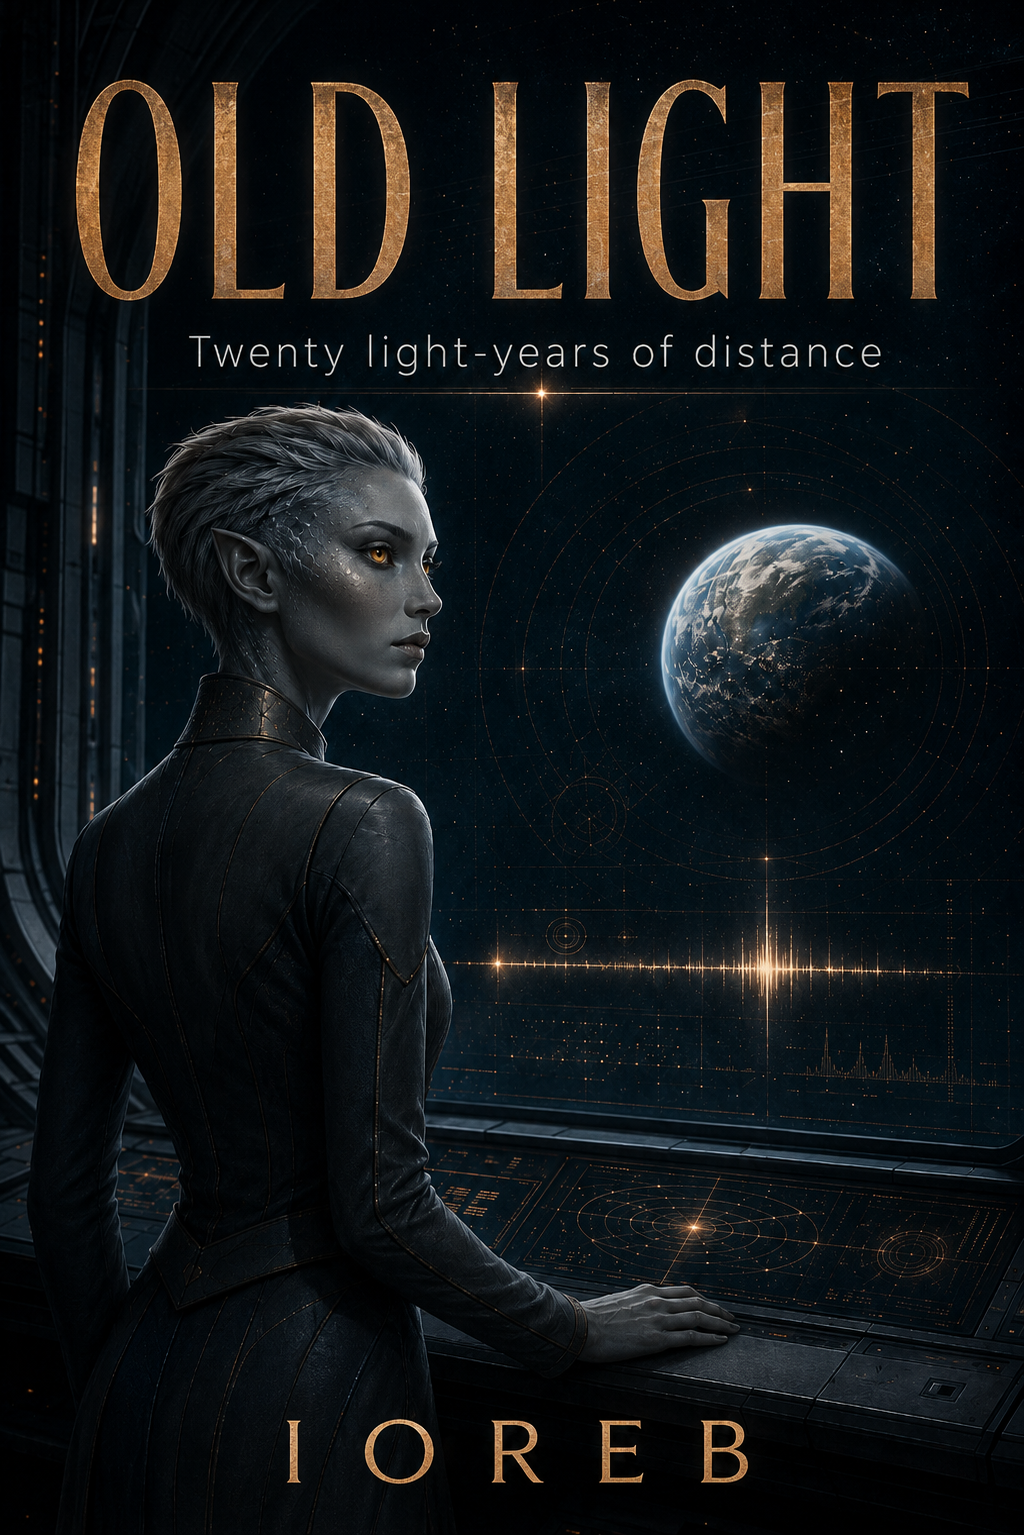
\includegraphics[width=\paperwidth, height=\paperheight]{portada_en.png}
\clearpage
\restoregeometry

\frontmatter
\maketitle
\clearpage
\thispagestyle{empty}
\vspace*{\fill}
\begin{center}
{\small
\textbf{Old Light} \\
Author: IOREB \\
© 2026, IOREB. All rights reserved. \\
\vspace{1.5em}
No part of this publication may be reproduced, distributed, or transmitted in any form or by any means, including photocopying, recording, or other electronic or mechanical methods, without the prior written permission of the publisher, except in the case of brief quotations embodied in critical reviews and certain other noncommercial uses permitted by copyright law. \\
\vspace{1.5em}
Cover design by: IOREB. \\
\vspace{1.5em}
AI Assistance Declaration: This work of science fiction was developed and translated with the assistance of artificial intelligence language models as part of an iterative agentic creative process at EditorIAl IOREB.
}
\end{center}
\vspace*{\fill}
\clearpage
\tableofcontents

\mainmatter
\chapter{The Weight of Silence}
\markboth{The Weight of Silence}{The Weight of Silence}

The problem with interstellar silence, Seran thought as she crossed the observation bridge, is that it is not silence at all.

It was noise. Background noise, microwave noise, the constant hiss of the universe cooling since its birth. What most people called silence was actually the longest conversation in history, one where no one had yet said anything interesting. Seran had been listening for seventeen years. So far, the universe had only coughed.

She stopped in front of the glass panel and looked out.

The station orbited four hundred kilometers above Kael, the world that had made them. From here, the curvature of the planet was laid bare: a blue-green band of atmosphere, bands of clouds organized in spirals that climate models had spent decades trying to predict without complete success, and beneath all of that, invisible to the naked eye, the network of cities that blinked at night like an exposed nervous system. Seran had been born in one of those lights. Now she spent most of her time up here, looking in the opposite direction.

It was a choice her mother had never quite understood.

Kael revolved around an orange star—Aur, they called it, though its technical designation was a seventeen-digit number no one used in conversation—at a distance that had kept its oceans liquid for just over four billion years. The planet was smaller than theoretical models predicted as optimal for complex life, and yet here they were: two billion Kael'thin distributed across twelve continental federations, with their wars, their arts, their applied genomics, and their radiotelescopes pointing into the void.

Seran was one of those who pointed.

Up here, at an altitude of four hundred kilometers, the world lacked tension. Seran felt that sharp emptiness at the base of her skull once more—the persistence of a phantom limb searching for a north that no longer existed. On the surface, Kael’s magnetic field was an invisible anchor that ordered the world; a constant internal compass, the physical certainty of knowing where the planet tilted without having to think about it. It was not a mystical sixth sense; it was a biological river integrated into their nervous system, the very one pre-industrial navigators had used for millennia to plot routes across the oceans. Here, on the station, that internal architecture returned only a dull silence. Aerospace medicine manuals often stated that trying to describe this deprivation to a Kael'thin who had never left the surface was like trying to describe a new color. An impossible abstraction. Seran, watching the blinking lights below, understood that the manual fell short: it was a constant directional blindness, a mute hum that reminded her at every instant that she was out of her element. It was the hardest part of orbit to bear. That, and the absence of rain.

She picked up her tablet from the ledge where she had left it and checked the night records from the antennas. The Kael Orbital Radio Astronomy Facility—IORK, to everyone who had to mention it frequently—was a joint project of eight federations, which meant its funding depended on eight parliaments with eight different electoral cycles and eight different definitions of what constituted a "scientific result of public interest." Seran had learned to write progress reports that sounded promising without actually being so, a skill she had been told she would not need when she studied Astrophysics.

The night's records were the usual ones. Pulsars. Quasars. The background murmur. Nothing that had not been there before.

She slid her finger down the columns of data with the sluggishness of one acting out of habit rather than expectation, and was about to close the tablet when something made her stop.

\vspace{1.5em}
\begin{center}$\ast$\quad$\ast$\quad$\ast$\end{center}
\vspace{1.5em}

The star was a G-K type, almost exactly between those two classifications, approximately twenty light-years away. It had been cataloged for decades, perfectly ordinary: mass slightly lower than Aur, luminosity somewhat less, a planetary system that spectroscopists had confirmed eight years ago using the radial velocity method. Four planets detected, one of them in the habitable zone. Nothing special. The catalog was full of stars like that.

What was not in the catalog was what Seran had on her screen now.

The radio emission profile of that star was incorrect.

Not in a dramatic way. There was no pulsing signal with a message in Morse code. It was subtler than that, and precisely because of that, Seran spent ten minutes staring at it with the feeling that she was seeing something that should not exist: in the frequency range between 40 and 1500 megahertz, the star’s radio spectrum had peaks. Discrete, structured peaks, distributed in a way that known astrophysical processes did not produce. Stars emitted radio continuously and smoothly, following spectral distributions that physicists had been modeling accurately for a hundred years. This was neither continuous nor smooth. This had shape. It had internal structure.

Seran applied all the interference artifact filters she had available. The peaks remained.

She checked if any known background object—a distant pulsar, an active galactic nucleus—could be aligned with that direction and producing the signal. Nothing in the catalog.

The peaks were not periodic with respect to each other in any simple way, which ruled out a single rotating object as a source. They were rather a superposition of multiple emitters: something producing radio on several frequencies simultaneously, with intensities that varied independently. It was almost like... structured noise. Noise that had been modulated by something before being emitted.

Seran stood still in front of the glass panel for a long time. Outside, Kael kept turning with its usual indifference.

\textit{It is probably interference from one of our satellites,} she thought, forcing the most boring hypothesis. Always the most boring one first.

But IORK's satellites had registered frequencies, and none matched the peaks she was seeing.

She tagged the entry in the log with maximum analysis priority. She did not alert anyone yet.

Then she closed the tablet. Then she opened it again.

\chapter{The Curvature of Lost Time}
\markboth{The Curvature of Lost Time}{The Curvature of Lost Time}

The Northern Kael Institute of Theoretical Physics occupied a building designed in an era when architects still believed that form should communicate content. It was a low, horizontal structure, built of gray delta stone, with long, narrow windows that let in Aur’s light at angles calculated so that the offices were never completely in shadow nor completely illuminated. Someone with plenty of time and a certain tendency toward symbolic interpretation might have said the building looked like an object on the boundary between two states. The physicists who worked inside usually said simply that it was cold in winter.

Tael arrived twenty minutes early that morning, which was unusual even for him.

He had slept poorly. Not out of anxiety, or not exactly: it was more the feeling of having something in his head that did not quite fit, like trying to close a box whose lid will not shut because there is too much inside. The last three years of the project had been a sequence of successive approximations to a result that always seemed two steps away, and now, suddenly, the previous week's simulation had returned numbers that matched. Not approximately. Exactly.

Tael was a good enough physicist to distrust exact results.

He hung up his coat—it was cold, as always in winter—and turned on the terminal before taking off his scarf. The files for the simulation remained open where he had left them the night before. He looked at them with the dense stillness of one who expects to find the error he knows must be in there somewhere.

The numbers still matched.

\vspace{1.5em}
\begin{center}$\ast$\quad$\ast$\quad$\ast$\end{center}
\vspace{1.5em}

The project had a long official name that no one used and an informal name that everyone used: The Bubble. It had started, like many theoretical physics projects, as an unintended consequence of another line of research. Twelve years ago, a team from Southern Kael had been studying the properties of space-time metrics in the presence of negative energy densities—a dark and technical field that at the time seemed interesting mainly to specialists in general relativity and no one else—when one of its members, almost in passing, had published a paper calculating the energy cost of creating a local distortion of space small enough that it contained no matter.

The paper had received few citations at first. Then, gradually, it had begun to accumulate them.

The problem with moving matter through metric deformation was both energetic and fundamental: the amount of negative energy required to create and stabilize a bubble large enough to contain even a gram of matter was astronomical in the most literal sense, and there were also causality objections that theorists had spent decades trying to resolve without clear success. But the Southern Kael paper had identified something else: a minimal-scale solution. A bubble so small that it could not contain anything with rest mass. A bubble that could not transport matter.

But it could transport a state.

The difference was subtle and took years to explain properly to non-physicists, but the core idea was this: information was not matter. A bit—a state, a yes or a no—weighed nothing. And if you could create a small enough and stable enough metric deformation bubble, the bubble could propagate through space carrying that state without violating any relevant conservation laws, because there was nothing inside to conserve. The bubble did not move matter. It moved geometry.

And geometry could move faster than light.

The problems were, of course, numerous.

The first was energetic: even at this minimal scale, the cost per transmitted bit was enormous compared to any conventional communication system. Not prohibitive—commercial fusion went a long way—but high enough that no one thought of using it to replace the planetary communications network. It was a technology with only one obvious use case: sending information across distances where the speed of light becomes a real problem.

The second was coherence: the bubble tended to deform during propagation, which corrupted the state it carried. It was like sending a letter inside an envelope that got wet during the trip. The three years of Tael’s project had been, in essence, the problem of finding how to waterproof the envelope.

And the simulation from the previous week said they had succeeded.

\vspace{1.5em}
\begin{center}$\ast$\quad$\ast$\quad$\ast$\end{center}
\vspace{1.5em}

Milen arrived at her usual hour, which was to say late, with a thermos container in each hand and that slightly tilted posture of someone who already senses there is news.

Milen was the co-director of the project, an experimental physicist compared to Tael's theoretical profile, and they had been working together long enough to have their own language made of silences and what kind of pause each made before speaking.

"They still match," Tael said without moving from the screen.

Milen placed one of the cups on his desk with the care of someone who does not want to celebrate too early.

"Did you find the error?"

"I searched for two hours."

"And?"

"It is not there."

Milen sat in the chair in front of his terminal—not her chair, but she had been sitting there frequently enough over the years for it to have taken her shape—and looked at the numbers.

"The phase correction term works," she said, in a low voice. It was not a question.

"The phase correction term works." Tael leaned back. "The bubble coherence remains above ninety-four percent throughout propagation to the limits of the model. With that fidelity rate, standard error correction protocols can recover the original state with no detectable degradation."

Milen said nothing for a moment.

The long, narrow window in front of her let in Aur’s light, which that morning was the color of old copper. Outside, the river delta surrounding the institute was covered in a low mist that slowly dissolved in the morning heat. Two large birds soared in circles over the water.

"How far?" she asked at last.

"The model scales up to three light-years with current parameters before degradation begins to exceed the correction threshold. With improvements to the containment generator, possibly ten."

"And the energy cost per bit?"

"At interstellar distances, roughly the equivalent of what a medium-sized city consumes during one second for every ten bits transmitted."

Milen weighed the figure.

"It is expensive."

"It is absurdly expensive for any ordinary communication. For interstellar communication, it is irrelevant. If there is ever something to send a message to several light-years away, the energy cost is not going to be the limiting factor."

"If there is ever something," Milen repeated.

It was the condition no one mentioned in the papers. The project had a name and it had funding and it made sense as fundamental research, but everyone on the team was mature enough to know they were building a technology for a conversation that might never take place. Sending information faster than light only mattered if there was someone on the other side who wanted to receive it.

And up to that moment, the universe had given no indication that anyone was there.

"We need to build the physical prototype," Tael said. "The simulation is not enough. We have to prove it in a real experiment, even at laboratory scale, even at a distance of one meter."

"That requires a new budget."

"Yes."

"How much?"

Tael passed her a sheet with the calculations. Milen read it. She held his gaze for the exact amount of time Tael had learned to decode as: \textit{more than we have, but less than I feared.}

"I will call the funding committee this afternoon," Milen said, rising. "I need you to prepare an executive summary for me that does not use the term 'negative energy density' in the first two pages."

"It is a necessary technical term."

"It is a term that makes the parliamentarians think of magic. Two pages, Tael. Then you can put in all the negative energy density you want."

Tael let his body lean back, evaluating whether it was worth objecting before deciding it was not.

"Two pages," he said.

Milen was already at the door when she turned around.

"Tael." A pause. "If this works in the prototype... how long until an actual operational system? Not the optimal model. The first one that is good for something."

Tael thought. It was the kind of question he preferred not to answer without numbers in front of him, but he knew the numbers by heart.

"Four years. Perhaps five, if the engineering of the generator is difficult."

Milen processed the information in silence, with the tension of someone doing arithmetic that had nothing to do with physics.

"Good," she said, and left.

Tael stared at the closed door for a moment. Then he returned to the screen.

The numbers still matched.

\vspace{1.5em}
\begin{center}$\ast$\quad$\ast$\quad$\ast$\end{center}
\vspace{1.5em}

That same night, four hundred kilometers above the planet, Seran was in IORK’s control room looking at the first data from the tracking session.

The anomaly was still there.

With forty-eight additional hours of integration time, the profile was now sharper, and sharper meant more impossible to explain comfortably. The spectral peaks in the radio range were not only confirmed: they showed a substructure that the first night's data had lacked resolution to reveal. There were patterns within the patterns. Modulations. The signal was not a single point source but something distributed—multiple overlapping emitters—and the frequency distribution had a shape Seran had been describing in her notes as non-thermal with complex structure, which was her way of writing what she still did not dare write in other words.

She opened the catalog of known interferences for the fourth time and scanned it for the fourth time without finding anything.

Then she did something she had been avoiding for two days: she searched SETI literature, the search program for extraterrestrial intelligence that the Kael'thin had been funding with varying enthusiasm for eighty years. She searched specifically for papers on radio signatures of technological civilizations. What they described as a detectable artificial signal.

The papers described exactly what she was seeing.

Seran closed the search. She stared at the blank screen for a minute.

Then she reopened it and kept reading.

\chapter{Unclassified Objects}
\markboth{Unclassified Objects}{Unclassified Objects}

The week of observation turned into three weeks without anyone formally deciding it.

That was how these things worked: Orath had said one week, and at the end of that week the data was strange enough that no one in the review room proposed stopping the observations, and since no one proposed it, the antennas kept pointing, and the data kept accumulating, and the week turned into two and then three with the same silent logic with which an interesting conversation extends past the hour when everyone had planned to go to sleep.

Seran had reorganized her routine without realizing she was doing so. She slept less. She ate in the control room more often than in the dining hall. She had three notebooks open simultaneously on her desk, and all three shared the same characteristic: the first pages were orderly, with numbered hypotheses and precisely cited data, and the most recent pages were a conversation with herself that had grown progressively less orderly as the data refused to resolve into anything simple.

The signal—they already called it the signal, in the control room, without capitalization but with the specific weight words carry when used to refer to something that does not yet have a name—was real.

This was no longer a hypothesis. It was a conclusion.

Preva had been the first to say it out loud, in the second week, with the flat tone of someone announcing a laboratory result without wanting the tone to add information the data did not yet justify: "The radio spectrum of that star is not consistent with any stellar emission model in the catalog, nor with parameter variations within physically plausible ranges. It is not natural noise." And then she had fallen silent, because what followed that conclusion was something no one wanted to be the first to write in an official document.

The third week's data had added the second piece.

Seran had coordinated with infrared observation satellites to point in the same direction. What she was looking for was the excess thermal emission: an active biosphere, an industrial civilization, both generate waste heat that escapes into space at infrared wavelengths. It was a weak signature at twenty light-years, at the limit of detectability with available instruments, but the data returned a clear excess. The planet—the third in the system, the one in the habitable zone—emitted more heat than could be explained by radiative equilibrium with its star.

Not much more. But more.

The kind of more produced by a planet with oceans, with continents, with an atmosphere that works. With life.

And then came the third piece, the one Seran had been waiting for without admitting she was waiting.

The planet rotated. And as it rotated, the intensity of the radio signal varied with a period of approximately seventy-one hours—the planet's sidereal day, Seran calculated, though she could not confirm it without more data—with a clear asymmetry: one hemisphere emitted more than the other. Not much more. But consistently so, session after session, with the regularity of something that was a structural property of the object and not a transient phenomenon.

One hemisphere noisier than the other.

Seran had written in her notebook, in very small letters, the two words that explained that. Then she had turned the page.

\vspace{1.5em}
\begin{center}$\ast$\quad$\ast$\quad$\ast$\end{center}
\vspace{1.5em}

The meeting in the third week was different from the previous ones.

The first two had the tone of an ordinary scientific review: data presentation, hypothesis discussion, action to follow. This one had something different in the air the moment Seran entered the room. It was something in the way people occupied their chairs—too still, too conscious of their own movements—and in the way conversations before the start cut off sooner than usual.

Orath was at the back of the room, standing in strict vertical alignment. It was his posture of \textit{this is important, I know, and I prefer to minimize my thermal footprint.}

Seran presented the data in order. The initial spectral anomaly. The forty-eight hours of tracking. The confirmation of the infrared excess. The rotational variability with hemispheric asymmetry. She did so without dramatizing, because the data did not need dramatization and because in her experience dramatization in science produced two equally useless reactions: either the listener got carried away by enthusiasm and stopped thinking critically, or they put themselves on guard against what they perceived as exaggeration and began looking for errors with more energy than necessary.

When she finished, there was silence.

It was Colm who spoke first.

"What is the hypothesis that best fits all the data simultaneously?" he asked. "Not the most probable. The one that fits best."

Seran did not need to think about it.

"A technological civilization on the habitable planet of the system," she said. "With radio emission sources non-uniformly distributed over the surface. Developed enough to generate detectable waste heat twenty light-years away. Whose electromagnetic pollution bubble is expanding at the speed of light and reaching our position."

The room absorbed the information in silence.

"How long has that bubble been traveling?" Verath asked.

"Twenty years, if the source is twenty light-years away. What we are seeing now is what they were emitting two decades ago."

"So they could be more advanced now."

"Yes. Or they might no longer exist. What we detect is old light. A photograph of the past."

"Could it be natural?" asked Rannek, the systems engineer, who had been silent until then. "Some mechanism we have not considered?"

"I have spent weeks looking for it," Seran said. "The radio spectrum is not reproducible by any known astrophysical process. The infrared excess in combination with that spectral signature has no natural analog in the catalog. And the hemispheric asymmetry rotating with the planet..." She paused. "...only something on the planet's surface that is not uniformly distributed can produce that. Nature can be many things, but it does not build radio transmitters that preferentially cover one hemisphere."

No one replied to that.

"We need the atmospheric spectrum," Orath said from the back.

"I know. That is the next step. If we get a direct spectroscopic observation of the planet during a transit, we can analyze the composition of its atmosphere." Seran had prepared this part. "If there is free oxygen and methane in proportions that cannot be maintained in equilibrium without a continuous source, it is an active biosphere. If there is also nitrous oxide or other compounds only industry produces, it is a biosphere with artificial chemistry." A pause. "The next calculated transit of the planet in front of its star is in thirty-eight days. I need to coordinate time on the high-aperture space telescopes."

"You have it," Orath said. Without deliberating, without conditions. Seran had been at IORK long enough to know that was unusual. "And I need someone to start thinking about protocol. If spectroscopy confirms what we are seeing, this stops being an internal research anomaly."

No one asked which protocol. Everyone knew what he meant: the eight federations that funded IORK, their parliaments, their ministries of science, and behind all that, the political structure of a planet that had never had to make a decision of this kind.

The meeting ended with the specific feeling that something had changed categories.

\vspace{1.5em}
\begin{center}$\ast$\quad$\ast$\quad$\ast$\end{center}
\vspace{1.5em}

Seran took a long time to leave.

Dovat stayed too. It was his habit: always the last to leave, as if the control room needed someone to lock up even though there was no key to lock it.

"Are you okay?" he asked when the others had gone.

"Yes." A pause. "I don't know."

Dovat accepted the pause in silence, as if the doubt itself were a completely satisfying answer.

"You have been searching for seventeen years," he said.

"Eighteen. The doctoral year counts."

"Eighteen." Dovat looked at the screen where the radio spectrum was still open. "How does it feel?"

"Like when you are reading a very long book," Seran said at last, "and you have been going for hours without anything happening, and suddenly on a page there is a sentence that changes everything you thought you knew about what you were reading, and you have to stop and go back and reread the previous pages with different eyes." A pause. "But I still don't know if it is that sentence or if I imagined it."

Dovat looked at the screen a moment longer.

"The transit spectroscopy will tell," he said.

"Yes. In thirty-eight days."

"And if it confirms?"

Seran closed the last notebook.

"Then," she said, "it stops being my discovery and begins to belong to everyone." Another longer pause. "And somewhere in that system, there is something that has been sending signals for decades without knowing anyone is receiving them."

Dovat said nothing. It was one of his best qualities.

\vspace{1.5em}
\begin{center}$\ast$\quad$\ast$\quad$\ast$\end{center}
\vspace{1.5em}

Eight hundred kilometers to the south and four hundred kilometers below, at the Institute of Theoretical Physics, Tael was still in his office at an hour when the building was empty.

The executive summary for the funding committee was finished. Two pages. No negative energy density on the first two pages, though there was on the third.

He thought, as he sometimes did when he was alone and the day had been long, about the question no paper mentioned directly but which was implicit in the entire project from the beginning: what is the use of a faster-than-light communication system if there is no one to talk to?

It was a rhetorical question. He asked it out of habit, not because he expected an answer.

He turned off the office light and went home.

Somewhere in Kael’s night sky, invisible to the naked eye, IORK kept listening.

And twenty light-years away, also invisible, a planet turned on itself in the darkness, spilling in all directions the noise of its own existence—televisions, radars, communication towers, the electromagnetic hum of a civilization that did not know anyone could hear—with the specific unawareness of one who has not yet considered that the silence of the universe might not be absolute.

In thirty-eight days there would be a transit.

These two things did not yet know each other. But the universe is small in ways people do not expect, and physicists and astronomers have annual congresses, and congresses have informal receptions where people talk about their work with a more relaxed rigor than in papers.

The next congress was six months away.

\chapter{Thirty-Eight Days}
\markboth{Thirty-Eight Days}{Thirty-Eight Days}

The thirty-eight days passed in different ways for different people.

For Seran, the thirty-eight days passed slowly, measured in the repetition of the same parameters. Fourteen times she opened the orbital file for KS-7741-b, hoping to find a deviation that the universe was not going to grant her. The planet would make its transit on the calculated date and not a second before. There was something cruel about astronomical waiting: the lesson that things happen at their own pace, a truth Seran believed she had mastered, but which forced her to stare at a screen that was not going to change until it changed all at once.

For Dovat, the days were measured in dry decisions. In the second week, when the director of a spectroscopic platform in Eastern Kael tried to withdraw half of their observation window to study a local magnetosphere, Dovat did not even raise his voice to answer the call. He opened the terminal, attached the complete table of priorities alongside the signal loss calculation, and wrote six words: \textit{If the transit fails, no retakes.} Fourteen minutes later, the window was confirmed on the schedule again.

For Orath, time fragmented into meetings where the air seemed denser. Before the scientific committee, he presented the data, omitting the third hypothesis—the one with a name—but letting the physics speak for itself. Later, before the twelve federations, he drafted a minute where a blank space occupied the place of the phrase \textit{artificial origin}. It was not an oversight; it was a silent invitation for the councilors to fill it in themselves.

For Preva and Colm, the wait was a battle against background noise. When Colm discovered the secondary modulation of less than a second and reached toward the internal alert control, Preva stopped his arm.

"No," she said, looking at the highly non-random graph. "Three more nights of data. If this becomes a rumor before the transit, it will be useless."

For Verath, the thirty-eight days passed in the past of others. He stacked eighty years of literature on his terminal regarding failed searches, biosignature models, and theories about civilizations that never gave signals. He reread articles that in their day seemed like pure speculation with the urgency of one seeking an instruction manual. By the third week, he realized he had spent days thinking of nothing else.

The transit began at four hours and seventeen minutes of IORK's night cycle, which was the moment the planet crossed the disk of its star as seen from Kael’s position, casting its shadow on the light that had been traveling for twenty years to the facility's instruments.

The entire control room was occupied. Seran had not formally summoned anyone—that would have been excessive for what officially remained a follow-up observation of an unclassified anomaly—but neither had she said she preferred to work alone, and the result was that by four hours and ten minutes there were eight people in a room designed for five, and no one had brought enough coffee.

The space telescopes began transmitting data in real time. On the room's central screen appeared the absorption spectrum of the planet's atmosphere: the chemical signature of everything between the star and them, printed on the light as a series of dark lines at specific wavelengths.

Seran had seen it hundreds of times on other stars, on other planets. It was always the same procedure: identify the absorption lines, cross-reference them with databases of known compounds, reconstruct the atmospheric composition. She had done it routinely for years. This time, her hands were not completely still on the keyboard.

The first results of the automatic analysis began to appear on her secondary screen. Seran read them. She reread them. She checked the calibration parameters of the instruments because that was what one did before declaring any result, not because she expected to find an error.

There was no error.

Molecular oxygen: 21\%. Nitrogen: 78\%. Argon: traces. Carbon dioxide: 0.04\% with a documentable upward trend in the historical data of the star itself collected over years. Methane: traces in proportions incompatible with thermochemical equilibrium in the presence of the detected oxygen, which was only possible if something replenished it continuously. Ozone: detectable layer. Nitrous oxide: present.

Seran stood still just long enough to finish reading the complete analysis.

Then she said, in a voice low enough to sound as if she were talking to herself, though everyone in the room could hear her perfectly:

"It is a biosphere."

No one said anything for several seconds.

"The oxygen and methane together are incompatible with abiotic chemistry," Seran continued, in the tone of someone providing context because that is what scientists do, even though the context in this case was almost redundant. "There is something alive there that produces methane continuously. The ozone indicates active photosynthesis or a functional equivalent. And the nitrous oxide..." She paused for a moment. "...the nitrous oxide has natural sources, but in these proportions, combined with everything else, it is consistent with intensive agriculture or industrial processing of nitrogen."

"How consistent?" Preva asked.

"Very."

Silence.

"And the radio signal?" Colm asked.

"The radio signal has been inconsistent with any natural source for three weeks." Seran looked away from the screen and faced the room. "This confirms it. We are not seeing two independent anomalies. We are seeing the same thing from two different angles."

Orath stood at the back of the room, as always. His hands rested at his sides, not crossed, not leaning on anything. It was a posture Seran had not seen in him before and took a moment to identify: it was the slight physical disorientation of someone whose magnetic anchor had just lost its north because what he was experiencing had no established protocol.

"When will we have complete data from the transit?" Orath asked.

"The full spectral analysis will be processed in four hours. But the preliminary data is already clear enough." Seran searched for the words she had been preparing for days without wanting to admit she was preparing them. "There is no interpretation of this data that does not include life. And the combination with the radio signal has no explanation that does not include technology."

Orath held eye contact long enough to confirm receipt.

"I am going to make some calls," he said, and left the room.

The next four hours were strange in a way that was hard to articulate.

The data kept coming. The instruments worked perfectly. The analysis progressed with the impassive mechanics of automated processes, indifferent to the weight of what it was calculating. In the control room, people spoke in low voices and did their work with a concentration that had something deliberate about it, as if keeping attention on technical procedures was a way to avoid getting lost in what the technical procedures were confirming.

Seran worked. She reviewed the spectral analysis layer by layer. She documented everything with the specific meticulousness of one who knows this document will be read by many people in many contexts for a long time. She wrote technical notes, described calibration procedures, calculated error margins. It was familiar work, and familiarity was an anchor.

Sometime between two and three hours of processing, Dovat put a cup of something hot on her desk without saying anything and left. Seran drank it without looking at what it was.

When the complete analysis was ready, she reviewed it one last time from beginning to end. Then she stared at the summary on the screen.

The planet had a diameter of approximately 12,700 kilometers. Average density consistent with a rocky world with a metallic core. Estimated surface gravity slightly lower than Kael's. Average surface temperature compatible with liquid water. Atmosphere with the composition of an advanced active biosphere.

And non-natural radio emissions that had been traveling toward them for at least twenty years.

Seran opened a new document on her terminal. At the top she wrote: \textit{Preliminary Characterization Report — Object KS-7741-b}. The name was the one the automatic cataloging system had assigned to the signal when Seran had first registered it, over a month ago. KS for Northern Kael, 7741 for the order number in the anomaly catalog of the year, b for the second entry of that observation session.

It was a very small name for what it designated.

She thought about changing it. Then she left the cursor blinking over it for a moment and decided it was not the time for names. Names would come later, when there were more people involved and more context and more time to think about what kind of name was appropriate for the first signal from another world.

She began writing the report.

\vspace{1.5em}
\begin{center}$\ast$\quad$\ast$\quad$\ast$\end{center}
\vspace{1.5em}

Eight hundred kilometers to the south and four hundred below, Tael was in the hardware laboratory when his terminal rang.

He did not hear it. He had spent two hours adjusting the parameters of the first physical component of the containment generator—a piece of hardware whose manufacture had required three months and two specialized suppliers—and the laboratory had the kind of active silence precision instruments produce, full of technical sounds that were not silence but trained the attention to ignore them. The terminal rang three times before Tael noticed there was something outside the usual pattern.

It was Milen.

"The committee approved the budget this morning," she said, without preamble. "Level B, not the Level C we asked for, but with an option for upward revision if the first results of the prototype are positive."

Tael set the instrument on the table with the care of someone who has learned not to drop things when receiving news, good or bad.

"Level B is enough to build the complete prototype."

"Yes. It is not enough for the final operational system, but the prototype, yes. How much time do you need to have the generator ready for the first coherence test?"

Tael looked at the piece on the table. He looked at the rest of the components arranged on the workbench with the precise geometry he had assigned them the previous week.

"Six weeks if all goes well. Eight if not."

"Four months for the full test, then."

"Three if the phase coupler engineering is cleaner than I expect."

"Good." Milen had something in her voice that Tael had learned to recognize as the contained version of a more intense mood. "The astrophysics congress is in five months."

"I know."

"It might be a good time to present the preliminary results. If we have them."

"We will have them."

A silence ensued. Not the kind that indicated there was more to say, but the kind that indicated what had to be said was difficult to formulate.

"Tael," Milen said. A pause. "Did you see the academic news this morning?"

"No. I have been here since six."

"There is a rumor. Nothing official, nothing with sources. But someone on the academic network is saying IORK has unpublished data on something unusual. An astronomical anomaly, without further details. I do not know if it is anything. But the astrophysics congress is where it will be known, if there is anything to know."

Tael looked at the generator piece.

"Do you think it is relevant to us?"

"I do not know. Probably not. But if there is something strange out there and it turns out we have the only technology that would allow us to do anything about it in less than several generations, we might be relevant to them."

Tael did not respond immediately. It was his habit when something deserved to be thought about before being spoken.

"Four months," he said at last.

"Four months," Milen agreed.

The call ended. Tael looked at the dark terminal for a moment. Then he went back to the workbench and picked up the instrument where he had left it.

Outside, over the delta, Aur was sinking toward the horizon. In the sky that was beginning to darken, the first stars appeared one by one, with the silent punctuality of things that have been there much longer than anyone has been looking at them.

\vspace{1.5em}
\begin{center}$\ast$\quad$\ast$\quad$\ast$\end{center}
\vspace{1.5em}

That night, Seran finished the preliminary report at two hours of IORK’s artificial cycle.

She reviewed it one last time. She corrected three typos and rephrased a paragraph in the conclusions that had sounded more categorical than the data justified. The final version was cautious in tone and forceful in facts, which was exactly the combination she wanted: so no one could say she had exaggerated, and no one could say she had not seen what she had seen.

In the conclusions section, she wrote:

\textit{The data obtained during the transit of KS-7741-b in front of its primary star, in combination with the radio spectral observations accumulated over the last nine weeks, are consistent with the presence of an active biosphere and a technological civilization in an industrial or post-industrial stage of development. In the opinion of the observing team, there is no hypothesis of natural origin that simultaneously explains all observations. It is recommended to open a protocol for continued observation and to notify the appropriate bodies in accordance with the established procedures for first-category findings.}

She saved the document.

She stared at the screen for a moment with her hands in her lap.

Eighteen years.

She did not think of anything in particular. It was not a moment of euphoria or fear but of something simpler and harder to name: the feeling that the world existing at that moment was fundamentally different from the one that had existed that morning, and that this difference could not be undone, and that this was correct even if she did not yet know exactly what it meant.

She turned off the secondary screen. She left the main one on, with the transit data open, because it felt wrong to turn it off.

Then she put on her coat and went to the observation bridge.

Kael turned outside, full of people sleeping without knowing. Aur had risen in the day hemisphere and its orange light arrived indirect, bounced by the planet’s atmosphere in a spectrum that the Kael'thin eyes found more comfortable than blue light. Seran looked at the dark sky in the direction where she knew the source lay, though there was nothing to see with the naked eye, though the distance made invisible anything that was not a star and the star in question was too dim to be distinguished without instruments.

Twenty light-years.

Out there, right now—in the moment that would be \textit{now} when the light leaving at this instant arrived at its destination twenty years later—there was something living and building and emitting signals without knowing anyone was receiving them.

Seran thought about that for a while.

Then she thought about the astrophysics congress, which was in five months, and all the conversations she was going to have to have before then, and that tomorrow she would have to start having them.

But that was tomorrow.

For tonight, the observation bridge was empty and the universe was slightly different from what it had been, and Seran allowed herself to be alone with that for a little while longer.

\chapter{The Congress}
\markboth{The Congress}{The Congress}

The Southern Kael city hosting the annual astrophysics congress was called Oru, and it possessed the kind of beauty river ports produce when they have been important for enough centuries: an accumulation of architectures from different eras that had not tried to coordinate with each other and yet for some reason worked together, like a long conversation between people who disagree on everything but listen to one another.

Seran arrived the day before her presentation, late enough that the hotel was almost empty of other congress attendees, and early enough that she could walk along the river promenade before it grew dark. She needed to walk. She had spent three weeks at IORK without coming down to the planet, and Kael's surface—the slightly higher gravity, the active magnetic field against her senses, the smell of the river—returned something to her she had not realized she missed until she had it back.

Kael's magnetic field was calm that night. No storms, no disturbances. A clean and constant orientation Seran felt as a gentle pull northward, so familiar she normally did not perceive it consciously, but after weeks in orbit, it was extraordinarily comforting. It was the feeling of knowing exactly where she was in the world.

If only everything else were as simple to locate.

The presentation was prepared. It had taken her two weeks to write it and three days to convince herself it was ready, which was unusual for Seran, who did not normally have trouble with presentations. The problem was not technical. The data was the data, the analysis was the analysis, the methodology was solid and documented. The problem was one of framing: how do you present something of this nature to a room of two hundred scientists without the weight of what it implies crushing the structure of what can be asserted with certainty?

She had decided, after much deliberation, to do it exactly as she would have presented any other result. With the data first. With the alternative hypotheses honestly examined. With the conclusions at the end, formulated with the exact precision the data allowed, adding nothing and taking nothing away. And let the room reach the implications on its own, because the room was perfectly capable of doing so.

What she could not control was what happened next.

The congress began the following morning with the usual plenary session: the president of the organizing committee, a summary of the year in astrophysics, three presentations of high-impact results that had come out in the last twelve months. Seran listened with half the attention she would normally have dedicated, sitting in the seventh row with the program in her hand and the feeling that time was passing in a slightly unreal fashion.

The afternoon session was where her presentation lay.

Orath was in the eighth row, three seats away from Seran. They had greeted each other that morning with the brevity of people who had spoken so much in recent weeks that they no longer needed preambles. Dovat had not come—someone had to keep operating IORK—but he had sent a message the night before that read simply: \textit{The data is correct, the methodology is correct, you are correct}, which Seran had saved in the folder of messages she never deleted.

Preva and Colm were in the fifth row. Verath, who had spent the last month becoming the foremost expert on atmospheric biosignatures among the Kael'thin, was in the second, with a notebook full of notes that Seran had been able to partially see the night before at dinner and which contained more questions than answers, which seemed to her exactly appropriate.

The session moderator introduced her with a description that read \textit{high-priority spectral anomaly, KS-7741 system} and nothing more, because Seran had expressly asked that there be no further context in the introduction. She wanted the room to reach the conclusions by reading the data, not by reading the title.

She stood up. She went to the podium. She looked at the room.

Two hundred people, approximately. The largest concentration of Kael'thin astrophysicists of the year in a single place. People who had spent their careers looking at the universe with different instruments and different questions, and who shared the same fundamental understanding of what constituted evidence and what did not.

It was the right audience for this. Probably the only right audience.

"The KS-7741 system," Seran began, "is a G-K type star approximately twenty light-years from Kael. It was cataloged decades ago as an ordinary system with four planets detected by spectroscopy. The third planet is in the habitable zone. Until nine weeks ago, there was no reason to pay special attention to it."

She paused. Not for dramatic effect, but because the next sentence required the room to be completely attentive.

"Nine weeks ago, during a routine review of night logs from IORK, I identified an anomaly in the radio emission profile of this star."

She projected the first graph. The radio spectrum, with the peaks marked, with the reference lines of known astrophysical processes clearly below what was observed.

She continued.

It took her twenty-two minutes to present the complete data, but she did not try to reinvent it before the room. The radio spectrum, the rotational variability, the infrared excess, and the transit appeared as a chain of failed refutations: each boring hypothesis had been tested, and each had left something more uncomfortable standing.

The room listened with a stillness that had nothing passive about it.

When she reached the spectroscopic analysis of the transit, Seran noticed the collective shift before finishing the sentence. Some hands stopped taking notes. Several glances shifted toward Orath, not toward her. From that point on, the presentation was no longer just scientific; everyone in the room was calculating which institution would have to make itself responsible for the conclusion.

"The atmospheric composition of KS-7741-b," she said, and projected the table of results, "shows free oxygen, out-of-equilibrium methane, ozone in a detectable layer, and nitrous oxide in concentrations consistent with biological or industrial processes. The combination has no known abiotic mechanism."

She let the table remain longer than usual. She did not need to repeat what anyone in that room could read.

She projected the final slide. It was text: the conclusions of the preliminary report, the same ones she had written at two in the morning weeks ago.

"In combination with the non-natural radio emissions documented over nine weeks, these data are consistent with an active biosphere and a technological civilization on the third planet of the KS-7741 system. In the opinion of the observing team, there is no hypothesis of natural origin that simultaneously explains the entirety of the observations."

Seran left the conclusions on the screen.

"I will be happy to answer questions."

The silence lasted four seconds. Seran counted them.

Then the room began to speak.

Not all at once, not with the chaos of an overwhelming emotional reaction. It was something more orderly and more intense: the simultaneous activation of two hundred scientific minds applying themselves to the same problem, producing the specific sound of many technical conversations starting in parallel. Someone in the third row had a question about the calibration of the spectroscopy instruments. Someone further back wanted the raw data from the radio analysis. An astronomer from Eastern Kael whom Seran knew from previous congresses raised her hand to point out a possible source of contamination in the infrared spectrum that Seran had considered and discarded but which was worth discussing in detail.

Seran answered everything. One question at a time, with the same precision with which she had presented the data. When she did not have the complete answer, she said so. When someone pointed out an alternative she had already examined, she explained why she had discarded it. When someone pointed out an alternative she had not considered, she noted it down and said she would examine it.

The question session lasted forty minutes, twice the allocated time. The moderator extended it twice without anyone protesting.

At the end, when the moderator terminated the session with the usual formula, there was something unusual: applause. Not the polite, quick applause that ended most presentations, but something more sustained and serious, the kind of recognition the Kael'thin scientific community reserved for moments when someone had done something everyone recognized as important.

Seran stood by the podium and thought, somewhat incongruously, that she wished Dovat could have been there.

The reception on the first night of the congress took place in a building by the river whose windows overlooked the water, and which at that time of the afternoon received Aur’s light at an angle that turned the river's surface into something resembling molten copper. It was the kind of setting organizers of scientific congresses chose deliberately to produce a mood conducive to conversations that mattered, and it worked despite the fact that all attendees knew perfectly well it was deliberate.

Seran had been at the reception for forty minutes and had had sixteen conversations, of which four had been substantial and the rest had been variations of the same exchange: someone would approach her, say some version of \textit{your presentation was extraordinary}, and Seran would reply with some version of \textit{the data is what it is}, and then the conversation would drift toward technical details, which was where Seran felt most comfortable.

It was not that she did not care about the recognition. It was that she still found it hard to separate the recognition from what had produced it, and what had produced it was still too big for personal recognition to feel like the important part.

She was in a moment between conversations, standing by one of the windows with something that was not exactly wine in her hand, looking at the river, when Verath appeared at her side with the expression of someone bringing someone else for a specific purpose.

"Seran," Verath said, "there is someone who wants to meet you. He says his work may be relevant to what you presented today."

"Everyone says that tonight," Seran said, without bitterness.

"He probably means it." Verath gestured toward his companion. "Tael. Theoretical physics, Northern Kael Institute. He has been working on a project about faster-than-light communication for three years."

Seran looked at the man Verath had brought. He was of middle age, with the sensory isolation of someone who had spent hours in a social space when he would prefer to be in a laboratory, and who held his own glass with the same reluctance Seran held hers. He wore a jacket that had been ironed several days ago and had decided on its own to relax the wrinkles since then.

Seran knew that kind of jacket. It was the jacket of someone who did not come to congresses for the receptions.

"Faster-than-light communication," Seran repeated.

"Yes." Tael had the voice of someone who had explained his work many times and had learned to do the short version. "Metric deformation at a minimal scale for state transport. No matter. Only information. The energy cost is manageable with commercial fusion. The coherence problem is resolved in simulation, and we are building the prototype."

Seran weighed that.

"At what distances?"

"The current model scales up to ten light-years with prototype parameters. With improvements in the containment generator, the theoretical distance has no intrinsic physical limit, only engineering constraints."

"Twenty light-years."

"With the technology we have right now, no. With an additional generation of hardware, possibly yes."

"How long?"

"Four years for the initial operational system. Perhaps three."

Seran looked at him for a moment. Tael maintained the same anchor of attention she recognized in herself when someone asked a technical question that deserved a technical answer: total focal isolation, without the magnetic noise of the reception.

"Verath," Seran said, without looking away from Tael, "can you get us something to drink that is not this?"

"I am sure it is not necessary for me to—" Verath began.

"Verath."

Verath registered the exchange with the stillness of someone who had done exactly what he intended to do, and went to fetch drinks.

They found a table in the least crowded corner of the room, next to a column that placed them partially out of the main line of sight of the reception. It was the kind of position two people choose unconsciously when they want to talk about something without the conversation being interrupted every two minutes.

Tael had brought a tablet with him, which at a congress reception was technically a violation of social protocol, but Seran was not the right person to point it out given that she had hers in the inside pocket of her jacket.

"How much do you know about what I presented today?" Seran asked.

"I have seen it all. I arrived this morning specifically for that. The rumor has been circulating on the academic network for weeks. I knew that if it was what it sounded like, the congress was going to be where it was confirmed."

"And?"

"It is what it sounded like." Tael placed his glass on the table. "I have a technical question about the spectroscopic analysis of the transit, if you do not mind. The nitrous oxide: did you calculate the isotopic ratio?"

Seran made a pause of deep recalibration. It was a good question. It was a very good question.

"Yes. The isotopic ratio of nitrogen-15 in the nitrous oxide is consistent with high-temperature biological production, not with natural atmospheric synthesis." She paused. "It was not in the presentation because it added a technical layer that would have slowed the structure of the argument. It is in the full report."

"Is it published?"

"Tomorrow. Orath sends it for review tonight."

Tael nodded. He took his tablet and opened something, then turned it toward Seran. It was a schematic diagram: a metric deformation geometry with mathematical annotations in the margins.

"The fundamental principle," he said, "is that a deformed metric bubble below the rest mass threshold can propagate at FTL speed without violating local causality because it does not transport any inertial reference frame. It only transports a state. The problem until three years ago was that the bubble degraded during propagation and the state arrived corrupted. We found the phase correction term that stabilizes coherence above ninety-four percent."

Seran looked at the diagram. It was not her field—she was observational, not theoretical—but the mathematics were legible and the structure of the argument was clear.

"What is the transmission rate?" she asked.

"In the prototype, on the order of hundreds of bits per second. With the next generation of generation technology, potentially kilobits. For sending a text message, it is enough. For sending a video, it is not."

"For a first contact, it is more than enough."

"Yes."

They looked at each other.

Outside, through the windows, the river remained molten copper under Aur’s light, which was now almost on the horizon. Somewhere in that same sky, invisible, KS-7741 emitted its ordinary light in all directions, including that of Kael, including that of this window, including the table in this corner where two people who had not known each other twenty minutes ago were having the most important conversation anyone had probably ever had on this planet.

"There is something I need to know," Seran said. "What we see in the radio signal has been traveling for twenty years. Those are emissions from twenty years ago. Can your system transmit twenty light-years with current technology?"

"No. With the current, ten light-years at most." Tael did not look away. "But the system is not physically limited by distance. Only by the power of the generator and the precision of the phase coupler. Both are engineering problems, not fundamental physics. With four years of additional development and adequate funding, twenty light-years is achievable."

"Four years."

"Perhaps three, depending on how the hardware scales."

Seran thought about this.

"What we are seeing now," she said, "are their emissions from twenty years ago. If we send them a message today, it will arrive in twenty years as well. If they reply the moment they receive it, their answer will arrive forty years after we send it."

"Correct. If you use light or radio."

"But if your system works at twenty light-years," Seran said, slowly, "the message would arrive in..."

"The transmission time is not zero. There is physical propagation, though FTL. At those distances, with the second-generation model parameters, on the order of weeks."

Seran set her glass on the table very slowly.

"Weeks."

"Weeks for the outgoing message. If they can reply in the same medium—and for that they would need instructions on how to build a receptor, which we could include in the message—weeks for the reply as well."

"Can you build the receptor with text instructions? With just a few hundred kilobits?"

"The receptor is the simplest part of the system. The basic schematic blueprints fit in less than a hundred kilobits with standard compression. But to ensure a signal crosses twenty light-years without dispersing, we will need to wrap that information in tens of terabytes of metric support. The Bubble needs data mass to be stable. If they have the physics, they will understand why. If they understand the mathematics of the message. If they are technologically advanced enough."

"They have been emitting radio for at least eighty years," Seran said. "Their oldest emissions that we have been able to detect in the background signal have that estimated age. Eighty years of radio technology implies an advanced industrial civilization." She paused. "And the isotopic ratios of nitrous oxide in their atmosphere indicate industrial agriculture. They are advanced enough."

Tael looked at her for a long moment.

"I need to tell you something," he said. "The congress has a theoretical physics session tomorrow afternoon. I had not planned to present. The prototype results are not ready yet."

"And now?"

"Now I think perhaps I should explain what we are working on. Not the results. The framework. The possibility. Because if you are going to open a protocol for continued observation and notification to political bodies, and if in three or four years someone is going to have to make a decision about whether we send a message and how, that decision is better made if the people making it know from the beginning that an option exists that does not involve waiting forty years for a reply."

Seran thought of Orath, the twelve federations, the parliaments with their electoral cycles.

"You are right," she said. "But you need to be prepared for tomorrow's session to change the nature of your project forever."

"I know."

"Do you have funding secured for the prototype?"

"Since this morning. Level B, with an option for upward revision."

"Then you have something to lose."

"Yes." Tael looked at her. "Did you have anything to lose this morning when you went to the podium?"

Seran considered the question.

"Eighteen years of work," she said. "My reputation if the data turned out not to be what it is. The possibility of remaining an ordinary astronomer with an ordinary career. Yes. I had things to lose."

"And?"

"And the data is what it is."

Tael pondered the statement in silence.

"The data is what it is," he repeated, as if it were a conclusion worth stating aloud.

Verath appeared at that moment with two glasses of something different and the relaxed posture of someone who had delayed deliberately to allow time for a conversation.

"Do I interrupt?" he asked, with a neutrality too elaborate to be genuine.

"No," Seran said. "Sit down. We need someone to remember this conversation in case either of us regrets it tomorrow morning."

Verath sat down.

Outside, Aur finished setting over the river, and the sky over Oru slowly filled with stars with the usual patience of the universe, which is in no hurry and which that night, as always, contained more than anyone looking at it could fully imagine.

\chapter{The Problem of Responding}
\markboth{The Problem of Responding}{The Problem of Responding}

Seran woke up knowing where north lay.

It was always the first thing she registered when returning to the surface, even before opening her eyes: Kael, constant and clean, returning a reference to her that in orbit became an absence. Three weeks on IORK were enough for that absence to become a dull background noise, something that did not hurt but never stopped. To feel the planet again was to recover a phrase in a language her body did not remember forgetting.

Beside her head, curled against the pillow with the precision of one who had found the exact spot where the world fit best, her treen slept. It was an old animal—she had owned it for eleven years—with dark, dense fur like that of an otter, a long body, and six tiny pupils closed in an irregular line. Its name was Orv, and it had a habit of sleeping aligned with her, generating a slight local resonance. It was not a sound. It was a sensation of being slightly more oriented than usual, as if the north were sharper near it.

Seran opened her eyes. The hotel room in Oru was functional and magnetically aligned—Southern Kael architecture always was—and Aur’s light entered the window at a low angle indicating early morning.

Her tablet was on the nightstand. The screen blinked with the cadence of accumulated notifications.

Seran ignored it for the time it took to sit up, scratch the back of her neck, and accept that the starting day was not going to resemble any other day of her life.

She picked up the tablet.

She had four hundred and twelve notifications.

It was not a number Seran's tablet had ever displayed. Most were requests for access to the preliminary report, which Orath had sent for review the previous night. There were requests from universities, regional observatorios, and institutions from three different federations Seran did not remember having active astrophysics programs. There were sixteen messages from science journalists, which was extraordinary because Seran did not know sixteen science journalists. There was a message from her mother that read simply: \textit{Is it true what they are saying on the news?} which Seran read twice before closing the application without replying—not out of discourtesy, but because she still did not know how to answer that question in a way that did not sound either too large or insufficient.

And there was a message from Orath, marked priority, sent at four in the morning.

Seran opened it.

The text was brief, with the economy of words Orath used when the situation was too serious for politeness: \textit{Secure line. Call me before speaking to anyone else. Not optional.}

Seran looked at Orv, who remained asleep with the absolute serenity of an animal that had no professional obligations.

"You stay here," she told it.

Orv did not respond. Seran dialed Orath's secure line.

The conversation lasted eleven minutes. When it ended, Seran sat on the edge of the bed with the tablet resting on her knees and her gaze fixed on the opposite wall, which had nothing special about it but served the function of being a place to rest her eyes while her mind assimilated a load of information that required all of its available capacity.

Orath had told her three things. The first was that the preliminary report had leaked to the public network before the review committee finished its evaluation, which was a protocol disaster but not a surprise: Seran had been suspecting for weeks that the academic network had more leaks than an old cooling system. The second was that news headlines in six federations already included some variation of the phrase \textit{we are not alone}, which was technically incorrect—the correct phrasing would have been \textit{the data is consistent with a technological civilization}—but Seran had stopped expecting journalistic precision at some point in her career.

The third thing was the one that mattered.

The Twelve Federations had summoned an emergency committee. Not a scientific committee. A political, planetary security, and interfederative coordination committee. And they wanted Seran to be present.

Seran had never been on a planetary security committee. She was not sure most people knew they existed. They were bodies activated for events that threatened the stability of the armed peace between federations: energy disasters on a continental scale, critical failures in the nuclear grid, the kind of things that occurred once every few decades and were managed in closed rooms by people who spoke in professional euphemisms.

The discovery of a technological civilization twenty light-years away had just entered that category.

"I am not a politician," she had told Orath.

"No," Orath had replied. "You are the person who has the data. And right now, the data is the only thing that can keep this conversation from turning into something no one is going to be able to control."

Seran looked out the window. Oru stretched under the coppery light of Aur, with its gray stone buildings aligned with the local magnetic field, with its wide river reflecting the sky like an old metal mirror. A city that had been important for centuries and would probably remain so when Seran was no longer here. A city that, like all cities on Kael, had been built by a species that took its time to do things, that thought in decades and centuries, that distrusted quick decisions because quick decisions were what had caused the Great Blackout and the Silent Wars and all that Kael had taken generations to repair.

And now that species had to decide, in a timeframe that was not going to be decades, what to do with the information that they were not alone in the universe.

Seran dressed, left food for Orv, and walked out of the hotel toward the council building without replying to any of the four hundred and twelve notifications.

\vspace{1.5em}
\begin{center}$\ast$\quad$\ast$\quad$\ast$\end{center}
\vspace{1.5em}

Orath had been working at the intersection of science and politics for forty-seven years, and he had learned two things most scientists never learned. The first was that truth, on its own, moves nothing; what moves is who controls the truth. The second was that the most dangerous crises are not those that cause panic, but those that cause silence.

The Oru council chamber was a polished stone amphitheater with perfect magnetic alignment—each seat aligned with the force lines of the local field, so that no delegate experienced the slightest physical discomfort they could attribute, consciously or not, to the environment rather than to the content of the discussion. It was an architectural detail Kael'thin diplomats had known for centuries: a magnetically misaligned room produced subliminal irritability. A perfectly aligned room produced clarity. Or at least eliminated an excuse for not having it.

Orath watched the delegates as they took their seats. He knew most by name, many by reputation, and some by the kind of knowledge acquired only after decades of institutional negotiations in which words mattered less than silences.

The delegates from the eight central federations arrived first, as usual. These were the federations that funded IORK, those with active scientific programs, those that considered investment in basic science as something a serious state had to do even if results took generations to materialize. They arrived with expressions Orath recognized: the controlled severity of people who knew they were facing something without precedent and who had decided, each in their own way, not to be the first to show it.

The delegates from the four peripheral federations arrived next. These were the far northern federations, those that survived on strict energy rationing, those that had spent decades arguing that resources destined for IORK were resources that did not heat the cities of the polar strip. Their expressions were different. They were not hostile—open hostility was rare in Kael'thin diplomacy, where strong emotions were considered a symptom of lack of control—but there was in them something Orath recognized from other difficult meetings: the patient hardness of people who have waited a long time for something to prove them right.

Seran was seated in the front row, in the place reserved for technical witnesses. Orath watched her for a moment. She sat straight with a controlled expression, applying all her discipline to the task of not looking as out of place as she felt. She was an astronomer in a room of politicians. It was not her element. But the data was hers, and in this room the data was the only currency everyone accepted.

The moderator opened the session with the protocol formula and yielded the floor to the lead delegate from Northern Kael, who was, by semiannual rotation, the coordinator of the committee.

The coordinator spoke for four minutes. He said the things that had to be said: that the session was extraordinary in character, that confidentiality was absolute, that the decisions made would have implications on a planetary scale. Then he asked Seran to summarize the data.

Seran stood up and presented the facts. She did so in seven minutes, half of what she had taken at the congress, because this audience did not need to have biosignatures explained to them. It needed to know what had been found, with what certainty, and what it implied.

When she finished, the silence was different from that of the congress. At the congress, it had been the silence of scientific minds analyzing data. Here, it was the silence of political minds calculating consequences.

The first to speak was Verath-Pol, the delegate from Polar North Kael, one of the four peripheral federations. He had a slow voice and the tone of someone who had learned to make criticisms sound like reasonable questions.

"How much has the detection of this signal cost so far?" he asked. "I refer to the cumulative cost of IORK over the last four years, including orbital maintenance, personnel, and energy consumption of the antennas. While in the polar north nodes we limit domestic thermal footprints during the winter cycle, here we seem to have energy to spare to listen to the void."

Seran looked at Orath. Orath silently authorized her.

"The operating budget of IORK is public," Seran said. "Approximately nine hundred million standard units annually among the eight sponsoring federations."

"Nine hundred million annually," the delegate repeated. "For four years. To listen to noise. And now that you have found something that is not noise, how much will what comes next cost?"

Orath intervened before Seran had to answer a question that was not really about money.

"The cost of continued observation is marginal," he said. "The infrastructure already exists. The relevant cost to discuss is that of the communication program."

"The Bubble?" said a delegate from Eastern Kael who had not spoken until then. "An experimental prototype from a theoretical institute that has not yet transmitted a single bit outside a laboratory? My nodes demand to know if the design of the phase coupler will be open source or if Northern Kael intends to retain the metric patent and the hardware contracts."

"A prototype with Level B funding and simulation results verified," Orath corrected. "And the only existing technology that allows us to contact a civilization twenty light-years away in a timeframe under forty years."

The debate continued for two hours.

Orath watched it as one watches a storm from a well-built building: knowing the structure would hold but alert for cracks. The positions were defined with the cautious slowness of a species that lived a century and a half and which visceral distrusted quick decisions.

The peripheral federations wanted a moratorium. They argued that the discovery was potentially destabilizing, that contacting a species whose electromagnetic emissions indicated a grotesquely inefficient energy use and an actively deteriorating atmosphere was, at best, premature, and at worst, dangerous. They invoked, without naming them directly, the Silent Wars. They invoked the Great Blackout. They invoked the principle that decisions with consequences spanning centuries required deliberations spanning decades.

The central federations were divided. Some supported continued observation but resisted funding the transition of The Bubble from an academic project to interstellar communication infrastructure. Others—the most industrialized, those with contracts with Tael’s institutes—saw opportunities that went beyond pure science.

Orath let the debate develop until the positions were clear and the fracture lines visible. Then he asked for the floor.

"The question before us," he said, with the calm and precise tone he had perfected during four decades of institutional navigation, "is not whether we must act. It is whether we can afford not to act. The signal exists. The data is published. The leak to the media has already occurred. Within six months, every citizen of every federation will know there is a civilization twenty light-years away. The question is not whether Kael responds. It is whether Kael responds in a coordinated fashion or if each federation acts on its own."

He let the implication settle.

"I propose the creation of a unified observation and communication program under interfederative supervision. Shared funding. Shared access to data. Political oversight by this committee. And the transition of The Bubble project from an academic program to state infrastructure."

"In exchange for what?" Verath-Pol asked.

"In exchange for total transparency," Orath said. "Every advance, every piece of data, every technical decision regarding the content of an eventual message will be subject to review by the committee. The academy will not act unilaterally."

It was a massive concession. Orath knew it. It meant yielding the control the Academic Pact had maintained for decades over fundamental research. It meant opening the doors of Tael’s laboratory to political inspectors and budget auditors.

But it also meant the project would survive. And that no single federation could monopolize it.

The vote was nine to three. The three peripheral federations that voted against demanded that their opposition be recorded in the minutes. No one was surprised.

Seran, seated in the front row, watched the result with the expression of someone who had just seen her scientific discovery definitively stop belonging to her and become the property of history.

Orath approached her when the session rose.

"Are you okay?" he asked, with the version of concern he used with people he respected, which was indistinguishable from pragmatism.

"I am trying to process it," Seran said.

"It will take you a long time," Orath said. "That is normal. The important thing is that the data is still yours. What we do with it from now on is everyone's responsibility."

Seran accepted the advice without looking away.

"Have you spoken to Tael?" she asked.

"No. Should I?"

"Someone should tell him that his laboratory has just become the most important facility on the planet. Preferably before he reads it in the news."

\vspace{1.5em}
\begin{center}$\ast$\quad$\ast$\quad$\ast$\end{center}
\vspace{1.5em}

Tael had spent three years working on a problem that, according to most of his colleagues, had no practical solution on a career horizon. It was the kind of work done calmly, with the methodical solidity of someone who knows he will not live long enough to see the final result but understands someone must lay the groundwork. He had adjusted his pace of life to that fact without drama, the way the Kael'thin adjusted almost everything: gradually, with decades of margin, without urgency because urgency was a luxury of species that aged fast.

What he had not adjusted to was the possibility of the pace changing.

Milen's communication arrived while he was reviewing the prototype's latest coherence logs, sitting at the only desk in the laboratory that had exact magnetic orientation—he had checked it himself with a magnetometer the day he arrived at the institute, eight years ago, and since then had not moved the desk a single centimeter. It was an uncomfortable desk, too close to the window in winter, but Tael had decided that comfort was negotiable and orientation was not.

Milen's message was text, brief, with the telegraphic syntax she used when she wanted him to read something without the additional nuances a voice could introduce: \textit{Vote approved. Unlimited funding. Committee supervision. The laboratory becomes state infrastructure. We need to talk.}

Tael read the message twice.

Then he set it on the desk and stared at the prototype's coherence data for a time he could not exactly quantify.

The problem was not the news. The news was, objectively, everything he and Milen had needed to take the project from where it was—a laboratory prototype that worked in simulation at ninety-four percent—to where it needed to be. Resources. Time. Engineers. Access to the containment generators of the industrial federations. Without that, The Bubble would have remained an elegant theoretical exercise for at least another decade.

The problem was the speed.

Tael understood the physics of metric deformation better than anyone alive on Kael. What he did not understand—what his brain, trained for eighty years to work in scales of decades, kept rejecting as an input error—was how to make a transition of that magnitude without making the process unrecognizable. A laboratory of six people that suddenly had to become a state facility with political supervision, electoral deadlines, and auditors asking about the cost of every meter of containment wire.

He had seen what happened to projects when politics adopted them. He saw them accelerate and fragment. He saw them produce results under pressure that later turned out to have cracks no one had had time to examine.

Milen entered the laboratory forty minutes later. She brought two cups of something hot and the expression of someone arriving with prepared arguments.

"I already know what you are thinking," she said, setting one of the cups next to Tael's desk.

"Then you save me time."

"You are thinking they are going to ruin the project with haste. That political deadlines are incompatible with the deadlines of physics. That we are going to end up building something that works seventy percent of the time and that no one is going to wait for us to be sure before using it."

Tael looked at her.

"Am I wrong?"

Milen sat on the edge of the table facing the desk—not the desk with perfect magnetic orientation, the other one—and held her cup with both hands.

"Probably not entirely," she said. "But the alternative was that they would fraction the project among three federations competing with each other to get there first. Orath has secured centralized supervision for us. A single committee, not twelve. It is imperfect. It is the best option available."

Tael considered this.

It was not that he did not understand. He had spent enough decades in academic institutions to know that pure funding, without political conditions, was a fiction that only existed in the opening speeches of congresses. What he struggled with was not the principle, but the scale of the change and, above all, the speed at which it was occurring.

His species was not designed for that. It was something he had read in evolutionary biology treatises but had never experienced with such clarity: the pressure of having to make important decisions in days when his nervous system had been calibrated for decades to make them in years. It produced a sort of cognitive hum, a background noise that was not exactly fear but was not anything else either.

"How much time do we have before the first committee supervisors arrive?" he asked.

"Three days." Milen set down the cup. "I know."

"Three days to document the current state of the prototype, the coherence verification process, and the scaling plan. In three days."

"Yes."

"That is absurd."

"Yes," Milen said, with the same equanimity with which she would have confirmed an experimental result. "But it is what it is. And you and I know that if we let the auditors arrive without documentation, they are going to interpret the vacuum as a problem. Do you prefer three days of intensive work or six months of audits?"

Tael picked up the cup from the table. The heat against his hands felt somewhat comforting.

"The coherence data is on the institute's servers," he said at last. "I can have the verification protocol documented in forty hours if Dovat lends us his analysis team."

"I have already asked Dovat. He said yes before I finished the sentence."

Tael looked at her for a moment.

"When did you decide all this?"

"During the vote. I knew you were going to need time to digest the political part. So I went ahead with the logistical part in the meantime."

It was, Tael thought, a perfectly accurate description of how they had always functioned. He found the phase correction terms. She built the scaffolding within which they could exist.

"Good," he said. "Forty hours."

Milen accepted the agreement and went to the other desk to open her tablet.

Tael stared at the coherence data for a moment longer. Ninety-four percent in simulation. Three years ago that had seemed extraordinary to him. Now, with the weight of what that number had to do in reality, it seemed fragile in a way he had not felt so clearly before.

But the data was the data. And the work was the work.

He picked up his tablet and began to document.

\vspace{1.5em}
\begin{center}$\ast$\quad$\ast$\quad$\ast$\end{center}
\vspace{1.5em}

The telepresence session with IORK began at sixteen hours, Oru time.

Seran had requested it before leaving the council. She needed to return to the data. Not the report data, which she already knew by heart, but the raw data: the original records of the signal, the unprocessed observations, the full radio spectrum of KS-7741 before any filtering algorithm touched it. She had spent hours in meetings with people talking about political implications and budgets and oversight frameworks, and she had the specific feeling of someone who had spent too much time at altitudes where the air was too thin: she needed to come down to something concrete.

Verath was already in the telepresence room when she arrived. He had his tablet open and an expression Seran recognized because it was the same one she had when she spent time looking at something that did not match.

"There is something in the rotation data," he said, without preamble, as soon as Seran sat down.

"The seventy-one hours," Seran said.

"The seventy-one hours." Verath turned the tablet toward her. "I have been looking at it while you were at the council. It does not match. It cannot match. A planet with that latitudinal temperature gradient and that mass distribution cannot rotate at seventy-one hours and maintain a stable atmosphere. Atmospheric dynamics models say that at that rotation speed thermal winds would have swept the ozone from the poles millions of years ago. And the ozone is there."

"I know," Seran said. "I noticed it when I reviewed the transit data, but I did not have an alternative explanation and did not want to include an unresolved inconsistency in the presentation."

"Well. Now we have time to resolve it." Verath opened the raw log. "Look at this."

It was the complete spectrogram of the observations of the last two months, unfiltered. Seran had seen it in its processed version hundreds of times. The raw version was different: noisier, with more structure, with overlapping signals that standard algorithms had discarded as interference.

"Do you see this pattern?" Verath pointed to a periodic modulation crossing the spectrum at certain intervals. "I had discarded it as contamination from a local source. But it is not contamination from a local source. I have checked against the catalog of all IORK objects. This pattern does not originate on Kael."

Seran looked at it for a long time.

"What is its period?"

"Approximately one hundred minutes. Very regular. Too regular to be a natural astrophysical process."

Seran calculated in silence.

"If there were a constellation of artificial objects in low orbit around KS-7741-b," she said slowly, "with orbital periods of around one hundred minutes, and if that constellation interacted with our observation windows..."

"They would produce a beat frequency," Verath completed. "An aliasing. The period we would measure would not be that of the planet's rotation, but the interference between the orbital cycle of the objects and the rhythm of our own observations."

"Calculate the beat frequency," Seran said.

Verath had already calculated it. It was evident he had calculated it before she arrived and had been waiting for the moment to show it to her.

"With an orbital period of ninety-seven minutes and our observation cadence, the resulting apparent period is seventy-one hours and four minutes."

Seran looked at him.

"And if you filter the aliasing?"

"With that as well." Verath slid his finger across the tablet and opened the corrected spectrogram.

The actual rotation period of KS-7741-b, once the effect of orbital interference was removed, was twenty-three hours and fifty-six minutes.

Seran said nothing for a moment.

Twenty-four hours. Approximately. One day.

Which meant that planet rotated four times faster than what they had measured. Which meant it was not the slow and marginally habitable world that atmospheric dynamics models had been trying to explain without success. It was a fast world. A world with short day-night cycles, with temperature gradients oscillating with a frequency that, on Kael, only occurred near the poles during equinoxes. Cycles that generated the winds that explained the polar ozone. Cycles that generated the meteorology that explained the dynamic cloud coverage. Cycles that explained, in fact, practically everything the models had not been able to explain using seventy-one hours.

And what the cycles did not explain, the other thing did.

"A constellation of artificial objects in a ninety-seven-minute orbit," Seran said. "How many objects would you need to produce that modulation?"

"To generate an interference of that amplitude and regularity," Verath said, "at least several hundred. Probably more than a thousand."

More than a thousand artificial objects in orbit around a planet. Each completing a revolution in approximately an hour and a half. A network. An orbital infrastructure of a density Kael had never had, Kael had never needed to have, Kael probably would not have for several more generations because Kael'thin space exploration was deliberate and cautious and did not put objects in orbit unless there was a precise and well-documented reason to do so.

Seran thought about what that implied. The kind of civilization that deployed more than a thousand artificial objects in low orbit around its own planet. Not as a massive, coordinated long-term effort, but as everyday service infrastructure, the way Kael deployed its communication networks on the surface.

A species that built that fast.

"Verath," Seran said. "When do you think they built that network?"

"Based on the evolution of the modulation intensity throughout the observations," Verath said, with the precision of one who had anticipated the question and had the answer ready, "the orbital density has increased steadily during the observation period. Twenty years ago, when the oldest emissions we have recorded began, the modulation was barely detectable. Now it is clearly visible. They have been deploying objects in orbit continuously for at least two decades."

Two decades of continuous orbital construction. More than a thousand objects.

Seran recalled what Tael had said at the reception the night before about the speed of construction and engineering deadlines. There was something in that moment of the conversation that now took on a different meaning: when she had asked how long it would take for The Bubble to reach twenty light-years, he had spoken of four years, perhaps three, as if that were a tight deadline.

For Kael, four years was a tight deadline. For a species that had been putting more than a thousand objects in orbit methodically and apparently continuously for two decades, four years was probably more than enough.

If that civilization received instructions to build a receptor, it would not take generations. It would not take decades. It would take the time it took to build infrastructure, and their relationship with infrastructure was not Kael’s: cautious, documented, with decades of testing before every step.

It was another one.

Seran did not know exactly what it was. She did not have enough data to characterize it precisely. But she had enough to know it was fundamentally different from theirs, and that this difference was going to be the most complicated problem of all the problems the discovery had generated.

Not how to talk to them. But at what speed.

"Note all this down," Seran said. "I want a complete report for Orath before tomorrow morning. And Verath."

"Yes?"

"Good job."

Verath held eye contact for the required second Kael'thin used to accept recognition without maximizing it, and returned to his tablet.

Seran stared at the corrected spectrogram for a moment longer. Twenty-four hours. A network of more than a thousand objects. A civilization that built as if time were a limited resource of which there was never enough.

\textit{We are not alone}, the headlines had said that morning.

It was true. But it was a statement that said very little about what it actually implied to be accompanied.

\chapter{Four Years}
\markboth{Four Years}{Four Years}

The phase coupler failed for the first time on day two hundred and eighty-seven.

It was not a spectacular failure. There was no overload, nor any of the dramatic ruptures the committee supervisors seemed to expect subconsciously when visiting the facility with their audit tablets. It was something much quieter: a number on Tael's screen that stopped matching the theoretical model. He stared at it with the unpleasant feeling that the room, usually aligned to the point of complacency, had tilted an impossible fraction toward an incorrect north.

"It does not scale," he said.

Milen, who was at the adjacent console reviewing the response of the metric tensor, stood up and approached his desk. On the screen, the scatter plot showed a clean drop. At four light-years, the signal coherence remained at ninety-six percent. At eight, it dropped to fifty-three. At twelve, the data packet turned into white noise.

At twenty light-years, the distance separating them from KS-7741, The Bubble simply did not exist.

"The interstellar medium is not homogeneous," Milen observed. Her voice did not change, but Tael noticed the minimal delay before each word. "The laboratory assumed an ideal vacuum. Reality has field fluctuations, charged dust, variable gas density."

"The correction term is insufficient by a factor of four." Tael slid his fingers toward the back of his neck. "If we cannot stabilize the phase against the inhomogeneity of the medium, The Bubble is just an expensive theoretical exercise with too large a committee."

Milen leaned against the edge of the table, staring at the vacuum between the consoles. She did not dispute the diagnosis. It was one of her virtues.

"The supervisors will come in three days. They will want to see a successful test transmission at full-range simulated scale."

"They will not have it. I am not going to falsify coherence data."

"I am not asking you to falsify it. I am asking you to find the adaptive term."

"We would need to map the actual stretch. Not a statistical approximation. The field, the gas density, the local discontinuities. Everything."

"Then we will have to convince IORK that an antenna that only listens is of no use if we cannot respond. I will handle the political management. You find the equation that corrects the phase."

Tael looked at her. Milen was already writing on her tablet, tracing lines of communication with the interfederative consortium, with IORK, with hardware suppliers who did not yet know they were going to lose the next few months of their lives. For Milen, physics was a constraint; politics was just another variable in the system.

"Eight months," Tael said at last. "If IORK gives us the field maps."

"Six."

"Eight, if we want it to work."

Milen stopped her fingers on the screen. Accepting a real deadline was, for her, a form of professional affection.

"Eight," she said.

\vspace{1.5em}
\begin{center}$\ast$\quad$\ast$\quad$\ast$\end{center}
\vspace{1.5em}

The next eight months did not take the form of discovery. They took the form of correction.

IORK yielded airtime no one wanted to yield. Preva constructed a noise map of the interstellar medium between Kael and KS-7741 from residue that previously would have been discarded as instrumental dirt. Dovat organized the flow of data between the orbital facility and the Node with the patience of someone who knows that technical miracles usually depend on no one mislabeling a file at three in the morning. Milen turned every administrative refusal into a partial concession. Tael stopped trying to find a clean equation and began looking for one ugly enough to describe reality.

He found it in the seventh month.

It was not elegant. It depended on an adaptive term that recalibrated during the initial propagation using an inhomogeneity matrix constructed from radio observations, polarized dust, and minuscule variations in the galactic background. Tael hated it for aesthetic reasons and defended it fiercely for physical ones.

The first full simulation returned a coherence of ninety-two point one percent at twenty light-years.

Milen did not celebrate. She opened another window and launched the simulation again.

The second returned ninety-two point zero.

The third, ninety-two point two.

Then Milen closed her eyes for the exact duration of a breath and said:

"Now we can have a moral problem."

\vspace{1.5em}
\begin{center}$\ast$\quad$\ast$\quad$\ast$\end{center}
\vspace{1.5em}

While Tael and Milen learned to send a geometry through a vacuum that was not a vacuum, Seran learned to look at a world that refused to order itself.

The intensive observation campaign had begun as a technical expansion of the original report and had become, almost without anyone deciding it, a new discipline. They were not studying a planet. They were studying the rhythm of a civilization.

The first thermal map showed five main continental masses, perhaps six if you counted the isolated polar mass. The third planet of KS-7741 did not have the broad, connected geometry of Kael, nor the distribution of oceans a Kael'thin climatologist would have considered reasonable. There were too many coastlines, too many fractures, too many thermal contrasts over short distances. It did not seem ugly to Seran. It seemed untamed.

The observation program also had a second, slower, and older component: the focal gravitational lens observatory, launched thirty-four years ago as part of the third SETI campaign. Until then, it had been dedicated to statistically promising targets. Following the discovery of KS-7741-b, the committee authorized its repositioning toward the Aur-KS-7741 line. It would take years to reach the useful geometry, but when it did, they would stop deducing continents from heat and start seeing light deformed by the star itself.

It was a patient instrument for a question that had stopped being patient.

The second week of radio analysis was worse.

Preva activated a reconstruction of the spectrum from the last decade. It was not the channeled pattern IORK's network produced. It was a superposition of independent emitters, overlapping bands, carriers stepping on each other, and protocols that seemed to have been designed by institutions incapable of waiting for others to finish.

"There is no global protocol," Preva said. "There are regions that ignore each other. Many. Some use the same frequency range with incompatible encodings."

"Competition?" Seran asked.

"Or political fragmentation. Or both. The signal does not allow us to distinguish."

Preva zoomed in on a broadband carrier.

"This is not telemetry. It does not seem like remote control either. It is a visual sequence."

"Visual?"

"Temporal images. Broadcast over the surface, not directed to a single node."

The reconstruction appeared on the console: an unstable, black-and-white frame crossed by interference lines. For three seconds, a bilateral structure formed, with two dark zones aligned on a moving surface. It was not geometry. It was not writing. It was not a map. The algorithm proposed a high probability of communicative anatomy, but did not dare classify it.

"It is repeated on thousands of carriers," Preva said. "We do not know if they are individuals, masks, rituals, or instructions. The only certain thing is that they transmit those shapes on a massive scale."

Seran watched the spot where the figure had dissolved. On Kael, information was delivered where it was needed. This was thrown into the air with an abundance that bordered on thermodynamic aggression. It did not look like a network. It looked like a fire with internal rules.

"And they are changing," Preva continued. "In the last four years of records, analog emissions are falling. Digital emissions are rising. They are replacing a planetary infrastructure while using it."

"Timeframe?"

"Years. Not generations."

Seran asked for the atmospheric data. Carbon dioxide kept increasing. Three percent in the last observed decade, with a trend that had no form of natural cycle. The same species that filled its low orbit with objects and its emission spectrum was altering the chemistry of its own air to feed that speed.

They were not observing a civilization in equilibrium. They were observing an organized combustion.

"If they receive blueprints," said Verath, who had not spoken for a while, "they will not wait a century to understand them."

No one needed to ask what he meant.

\vspace{1.5em}
\begin{center}$\ast$\quad$\ast$\quad$\ast$\end{center}
\vspace{1.5em}

The debate in the Message Committee lasted fourteen days and left Orath older than when he had entered.

The Oru chamber was perfectly aligned, but the tension between the delegates created a distortion no architectural design could correct. The question was no longer technical. The adaptive term worked. The Bubble could get there. What remained was to decide if it should.

"We are proposing to send blueprints of applied metrics," argued the Northern Kael delegate. "Not a philosophical formula. Not a greeting. A technology that deforms local space-time. To a species that does not coordinate its emissions, that fills its orbit with objects, and that alters its atmosphere as it accelerates."

"We are not sending them a transmitter," Orath replied. "We are sending them a receiver. An ear."

The polar delegate, Verath-Pol, did not accept the metaphor.

"An ear built with energy densities they have not shown they know how to handle. And once they have the receiver, they will have the principle. Their digital networks change at a speed we do not know how to audit. If they possess automated design systems, if they optimize without understanding, they could turn our blueprints into something else before they comprehend what they are touching."

That objection produced a heavier silence than the previous ones, because it was not a superstition. It was a reasonable extrapolation.

"They also might not build it," Seran said from the row of technical advisors. "Or they might build it poorly because they lack information. Or they might take decades to reconstruct what we have decided not to explain. All options carry risk."

"The option of not acting carries risk too," Milen added. "They already know how to emit. They have already filled their immediate environment with instruments. If they detect the radio shell and do not understand the metric, they will seek their own explanation. Fragmented. Militarized, perhaps. We cannot control what they will do with the silence."

"The Silent Wars started with technologies everyone considered manageable," Verath-Pol said. "Speed is not a virtue in itself."

"No," Orath said. "But neither is it a disease that disappears because we do not look at it."

Seran asked for the floor again. She did not look at the polar delegate. She looked at the center of the chamber, where the local magnetic field was most stable.

"What we see of them has a twenty-year delay. In forty years of radio round-trip, that civilization could have changed irreversibly. It could have collapsed. It could have learned on its own something worse than what we fear teaching them. The Bubble does not eliminate risk. It only reduces the time during which we are making decisions based on electromagnetic fossils."

She did not win the argument. No one won anything in that chamber.

What occurred was narrower: the committee accepted that the lesser risk was to speak.

Orath paid the price. The Academic Pact yielded total oversight of the message content, temporary freezing of patents derived from The Bubble, interfederative auditing of the budget, and shared access to all observation data. No single federation could monopolize the response. No single laboratory could act alone.

The vote was nine to three. The three peripheral federations demanded it be recorded in the minutes that they considered the decision premature, technically arrogant, and morally unstable.

It was decided that the message would be minimalist: a mathematical opening to demonstrate intent, a reciprocal observation block to show they were not speaking blindly, blueprints of the receiver with enough redundancy for an industrial species to build it, and deliberate silence about Kael. No history. No biology. No promises.

Only a physical bridge, and the limited hope that on the other side they would understand that a bridge does not force one to cross.

\vspace{1.5em}
\begin{center}$\ast$\quad$\ast$\quad$\ast$\end{center}
\vspace{1.5em}

Tael received the authorization three days later, at the Node.

He was alone in the control room, reviewing the data packet loading in the metric bubble one last time. Milen entered and stood by the door. On the main screen, the estimated coherence marked a stable ninety-two point one percent. Below, the trajectory model cut through the already mapped interstellar medium, with each adaptive correction waiting its turn like a sentence that had not yet been spoken.

"Are you ready?" Milen asked.

Tael did not look at the authorization screen. He looked at the line representing the path to KS-7741, a line too simple to contain four years of work, fourteen days of moral dispute, and twenty light-years of mutual ignorance.

"The system is ready," he said, and for the first time in four years, his voice did not sound like that of an engineer describing a machine. "The decision is not ours."

He pressed his thumb against the authorization sensor.

The loading sequence began.

\chapter{The Bubble}
\markboth{The Bubble}{The Bubble}

The orbital facility hosting the prototype of The Bubble had no official name.

The interfederative committee, at its first meeting after the approval of the unified project, had commissioned a naming process that had generated one hundred and forty-two proposals, three controversies over cultural representation, and a specific subcommittee to resolve the first two, and which four years later remained technically ongoing. The engineers who worked on it called it simply The Facility. The media, with the creativity that characterized Kael'thin science journalism, had called it the Node, and that name was the one that had survived in everyday language because it was brief and precise and did not imply any political position on which federation had contributed most to its construction.

Seran had arrived the previous afternoon. She had specifically asked to stay in the module furthest from the core, the one with the largest windows facing outward, because after four years of committee meetings in windowless rooms, she needed space to remind her why they were doing all this.

Kael was visible on the right, large and curved with its blue-green band of atmosphere. The stars were stars: with no atmosphere to diffract the light, no magnetic field to give them a sense of north, no spatial reference except pure physics and the geometry of space. Somewhere in that geometry, at exactly the distance their instruments had measured to four decimal places, was KS-7741.

And around KS-7741-b, without knowing it, a species that had been emitting radio for eighty years was about to receive something no one had ever sent them.

Seran did not sleep well. This was not unusual.

\vspace{1.5em}
\begin{center}$\ast$\quad$\ast$\quad$\ast$\end{center}
\vspace{1.5em}

The activation was scheduled for nine hours, IORK standard time.

Tael arrived at the control module at six. Milen arrived at a quarter past six. Orath arrived at seven with the representative of the interfederative political committee, a man named Verath-Pol who was different from the astronomer Verath of IORK—the phonetic coincidence had generated minor confusion for weeks in official communiqués—and who sat in silence in the observation seat at the back of the room and did not speak all morning, which Seran appreciated.

The Node's control room had space for twelve people. There were nine that morning: Tael, Milen, and the four main systems engineers at the operating consoles; Seran, Orath, and Verath-Pol in the observation seats. The rest of the team—forty-two people in total who had contributed at some point to the project—followed the activation from the adjacent monitoring room, where there were screens but no consoles, because this part of the process did not need more hands than those already in the main room.

Tael did not make speeches.

Seran had expected something—not a grandiloquent speech, that was no one's style in that room, but perhaps some formulation that marked the difference between this moment and the thousands of technical moments before. Instead, Tael simply said: "We begin the pre-activation protocol," and the engineering team began to work, and that was all.

The pre-activation protocol lasted forty-one minutes. It was a sequential verification of each subsystem: the containment generators first, then the calibration rings, then the phase coupler with the adaptive correction term loaded—the same term Milen had calculated and Dovat had verified, representing eight months of additional work that had turned a failed test into one that worked at ninety-two percent under real conditions. Each subsystem reported its status. Each status was recorded. No one spoke unless there was something technical to say.

Seran observed the screens from the observation seat. On the main screen was the status of the data packet: the message, compressed and verified and ready for encapsulation in the metric bubble. Fifty-three terabytes. The payload—mathematical index, reciprocal observation, and complete blueprints of the receiver—occupied a small fraction of the total; the rest was metric wrapping, redundancy, and error correction to maintain signal coherence across twenty light-years of interstellar vacuum. A colossal volume of structure for an idea to arrive without falling apart. The committee's information theory expert had described it with a contained emotion that Seran had found both surprising and completely appropriate.

At three minutes past nine, Tael said:

"All systems in green. Starting encapsulation sequence."

It was the moment when the data packet—the primes, the reciprocal observation data, the receiver blueprints, the calculated silence about everything else—was wrapped in the geometry of metric deformation. The process took four minutes and twenty-two seconds, during which the control room produced a specific sound that was not exactly silence but was the closest to it that a room full of people could produce: the deliberate absence of unnecessary conversation.

Milen followed the coupler readings with a concentration Seran recognized from the four previous years: the same she had had the night she found the correction term, focused on her tablet with her attention anchored slowly on the data.

At nine hours, seven minutes, and forty-four seconds, Tael said:

"Encapsulation complete. Initial coherence: ninety-three point one."

One point higher than expected. No one commented on this out loud. Milen recorded the data with the stillness of someone making a mental note of a result and moving on.

"Starting propagation."

The main screen changed. It no longer showed the packet status but the status of the metric bubble: a geometry the Node's instruments could detect during the first seconds of propagation before it reached a speed that left them out of range. The numbers changed fast. Tael read them in a low voice, not to inform anyone but with the mechanics of someone who needs to verbalize to process.

"Propagation speed: two hundred and forty-seven times c. Trajectory confirmed. Adaptive correction active. Coherence in margin..."

Seran had stopped her basal magnetic oscillation. She had not realized the rigidity of her anchor until she noticed it.

"...ninety-one point seven. Within parameters."

Four minutes followed in which the instruments detected the trace of the bubble moving away. It was a weak signal and faded rapidly, but while it existed, it was verifiable: the object they had built worked. It was propagating at the speed predicted by the calculated trajectory.

At fourteen minutes past nine, the signal disappeared from the instruments.

Tael confirmed it in the same voice he had used for everything before:

"Signal out of detection range. Nominal propagation. The encapsulation has left the Kael system."

No one applauded. It was not the kind of room where people applauded.

Orath, who had been silent all morning, said:

"How long until it arrives?"

"With current parameters," Milen said, "between sixteen and twenty-three days. The variability is due to the inhomogeneity of the interstellar medium in the final stretches of the trajectory."

"And if something fails in that stretch?"

"If something fails," Tael said, "we will not know. We have no way to verify the bubble's status once it is out of range. What we can verify is whether the receiver, once built, detects the packet or does not detect it."

"How long for them to build the receiver?"

No one answered immediately. It was the question no one in that room could answer with data, because the answer depended on something they did not know: the speed at which the other species functioned.

"Seran," Orath said.

"Based on the orbital construction speed we have observed," Seran said, "and on the amount of technical information we have included in the blueprints—and on the fact that they have computational tools we do not—between two and five years."

"Between two and five?"

"The uncertainty is about their will, not their capacity. If they receive the message and decide to build the receiver, they can do it. The question is whether they will."

Another silence followed.

Verath-Pol, who had not spoken all morning, asked from the back of the room:

"What do we do while we wait?"

Seran crossed her attention with Tael. Tael held the anchor.

"We watch," Seran said. "And in a few months, when the gravitational lens observatory reaches the focal line, we will stop intuiting them in the radio noise and see them with our own instruments. We keep watching. Now with more care than before."

\vspace{1.5em}
\begin{center}$\ast$\quad$\ast$\quad$\ast$\end{center}
\vspace{1.5em}

That night, Seran stayed in the module with the windows facing outward.

Kael remained visible on the right. The stars remained stars. Somewhere in the direction her instruments had verified, a fifty-three terabyte packet was traveling at two hundred and forty-seven times the speed of light toward a system that did not know they existed.

There was no way to know if it would arrive. There was no way to know if it would be received. There was no way to know if, in the event of being received, there would be anyone there who understood it.

What Seran did know was that, at some point in the coming weeks, the message was going to cross the heliopause of KS-7741's solar system. It was going to enter the space that civilization considered its immediate environment. And if there was any instrument in that system sensitive enough to detect the metric deformation of the bubble, it would detect it.

If there was someone looking.

Seran had spent eighteen years learning to listen to the silence. She had spent the last four learning to speak into it.

Now the only thing left was to wait and see if the silence answered.

\chapter{New Light}
\markboth{New Light}{New Light}

\textit{Epilogue to Part 1}

The fucking noise, Nadia Ostrova thought, rubbing her eyes as the gravel of the Parkes parking lot crunched under her boots. The problem with noise is that it never, ever shuts up.

It was one-fifteen in the morning in New South Wales. It was cold, the wind whipped her face, and the main radiotelescope—sixty-four meters of steel pointing blindly at the galactic plane—towered over her like a monument to sleep deprivation.

Nadia had been on leave for three months. "Acute stress, sustained exhaustion," her doctor in Sydney had diagnosed, looking at her over his glasses as if she were a reckless child and not a forty-four-year-old astrophysicist who had spent fifteen years listening to an empty sky. She had spent three months at her mother's house in Odessa, eating too much, sleeping at odd hours, and feeling the universe keep spinning without her.

Now she was back. And she had asked for the night shift because, frankly, it was the only one where she did not have to deal with the institute’s bureaucracy breathing down her neck.

She entered the control room. It smelled of overheated plastic, stale sweat, and the worst coffee in the Southern Hemisphere. Priya, the systems engineer, was typing frantically with his headphones on, nodding his head to the rhythm of something that sounded like industrial percussion. Tomás, the PhD intern, was snoring openly, sprawled across three folding chairs with a printed report stuck to his cheek.

"Tell me the network hasn't crashed again," Nadia blurted, throwing her jacket over the back of a chair and grabbing a paper cup from the machine. The black liquid that poured out tasted like burnt tire. Perfect.

Priya took off one earbud.

"All green, boss. Pulsars, quasars, and the same old boredom as always. Welcome to the vampire shift."

Nadia grunted something unintelligible and sat in front of her console. The monitor had a red dead pixel in the bottom right corner. It had been there for two years. She gave it a useless tap with her fingernail and began dumping the logs from the last eight hours.

Two hundred screens of white noise. Waterfall plots. Anomalies automatically discarded by filters.

She was about to pour herself another cup of tar when she saw it.

It was not an elegant epiphany. It was a stumble. Her eye jumped over a line in the data waterfall, her brain screamed \textit{error!} and her hand hit the spacebar so hard the keyboard creaked.

"Wait," she muttered, leaning in toward the screen until her nose almost touched it.

There it was. Forty to eighty megahertz range. Coordinates: Right Ascension 22h 14m, Declination +18° 42'.

A stupidly large amplitude peak. Ridiculous. Absolutely artificial.

"Priya. Pass me the local interference filter. Now," Nadia barked. Her pulse had just accelerated to one hundred and twenty beats per minute. The fatigue from her three months of leave evaporated instantly.

"What's wrong? Do we have a rogue Russian military satellite?" Priya typed fast.

"I wish it were a rogue Russian. Look at the spectral signature." Nadia pointed at the monitor with a trembling finger. "It doesn't fit. It's not GPS, it's not military X-band, it's not an ionospheric bounce."

Priya narrowed his eyes. He took off the other earbud.

"Shit. It has structure. Is there... is there phase modulation in there?"

"Cross-verify with the secondary dishes. Hurry up, damn it. Tomás!" Nadia kicked the leg of the intern's chair. "Wake up! Align the secondaries to sector 22!"

Tomás almost fell to the floor, blinking blindly under the fluorescent lights.

"What? What time is it?"

"It's time for you to justify your fucking scholarship!" Nadia was already opening three console windows at once, her heart pounding in her throat. "Priya, tell me the phase shift."

"Correlating..." Priya swallowed loudly. "Nadia... the time delay between the antennas gives a non-local origin."

Nadia stopped breathing.

"Extrasolar?"

"Confirmed. It's extrasolar. It's not coming from our system."

The room fell into a sudden, electric silence, broken only by the hum of the servers. The noise of humanity crashing against the wall of the impossible.

Nadia typed the coordinates into the cross-reference catalog. The server took three agonizing seconds to respond.

G-K type star. Twenty light-years away. Four planets. No pulsars. Nothing active. No excuses.

"Four minutes and nineteen seconds of log..." Nadia whispered, running her hands through her hair in desperation. "And then it disappears into the background. It's a pulse. A fucking coherent pulse."

"Nadia," Tomás's voice trembled. He had stood up. "Are you saying that is...?"

"I'm not saying anything until I have more data." Nadia turned to Priya, her eyes bloodshot, adrenaline burning through her veins. "Redirect the main dish. I want all available bandwidth pointing at those fucking coordinates. Call Canberra. Call the director. Get everyone with an access level higher than three out of bed."

"It's two in the morning, boss."

"I don't care if it's Judgment Day, Priya! Reorient the dish!"

The monstrous gears of sixty-four meters of steel began to turn in the darkness outside, groaning under their own weight.

Nadia Ostrova clung to the edges of the console. The dead pixel was still there, blinking red. But the universe had just turned on in every frequency.

\textit{End of Part 1}

\chapter{Background Noise}
\markboth{Background Noise}{Background Noise}

The dead pixel on the screen was still blinking red, a tiny factory defect in the bottom right corner. Nadia Ostrova had been ignoring it for two years, but now it seemed like the only fixed point in a room that had suddenly lost its gravity.

"Canberra on the line," Priya said, her voice an octave higher, her hands shaking over the keyboard. "The Tidbinbilla communications complex confirms they have their seventy-meter dish pointing at our coordinates. They are receiving."

"Time delay?" Nadia asked. The adrenaline scraped her throat like sandpaper.

"Identical. Extrasolar origin confirmed by two independent facilities."

Tomás, the intern who five minutes ago was sleeping on top of a report, pressed his fists against his thighs, his eyes wide open. The Parkes control room smelled of ozone, cold sweat, and a burnt coffee pot that no one had remembered to turn off.

Nadia leaned over the console. The data waterfall flowed on the main screen. It was no longer a simple pulse. It was something continuous, dense—an electromagnetic torrent sweeping through the galactic background noise with the brutality of a hammer.

"Run it through the spectrum analyzer. Heuristic mode," Nadia ordered. "Tell me what we're looking at."

Priya typed. The screen split. Lines of code began compiling the internal structure of the signal in real time. For ten agonizing seconds, the progress bar seemed to freeze. Then, the server spat out the result.

"It's binary," Priya whispered.

"The universe is full of binary things," Nadia said, though her heart was beating so fast she could barely hear her own voice. "Pulsars, white dwarfs, microwave echoes..."

"No, boss." Priya turned the monitor toward her. "It's math. Pure math. It's a sequence of prime numbers."

Nadia felt a physical shiver. The Wow! signal, the chimera of all SETI for half a century, had been a stupid alphanumeric pulse that never repeated. This was different. This was deliberate.

"[2, 3, 5, 7, 11]...?" Tomás asked, stuttering.

"No." Priya swallowed. "They are starting with huge Mersenne primes. They are sending the exponents in pure sequence. They are firing them one after another. It's... it's a beacon."

Nadia placed her hands on the desk. The wood was cold. The entire universe had just shrunk to fit into that room, but the planet kept spinning. And that was exactly the problem.

"Tomás," Nadia said, with a sudden, artificial calm. "How much time do we have left before the Earth's rotation puts us in the acoustic shadow?"

Tomás blinked, shaken from his stupor. He looked at the orbital tracking clock.

"Fifty-two minutes. In fifty-two minutes KS-7741 sets in the west and Australia loses direct line of sight."

Fifty-two minutes. In less than an hour, the Australian radio astronomy network would go blind and deaf to the area of the sky from where someone was shouting at them.

"We need someone in the other hemisphere to pick up the torch," Nadia said. She grabbed the landline phone on the console. The secure one, the one that did not go through the switchboard.

She dialed a number from memory. It was four-ten in the morning. The phone rang three times before a hoarse, grumpy voice answered at the other end.

"\textit{This better be the main dish burning down, Nadia,}" said Aris Thorne, Director-General of CSIRO.

"Aris, shut up and listen," Nadia said. "We have a coherent pulse. Confirmed by the Parkes main dish and the seventy-meter at Canberra. Extrasolar origin, KS-7741 system. Coherent emission centered at 1.42 gigahertz. The hydrogen line. It's a mathematical beacon. A sequence of primes."

Priya and Tomás exchanged a terrified glance.

Silence fell on the other end of the line. A thick silence, loaded with fifty years of false alarms, poorly calibrated microwaves, and military interference.

"\textit{Nadia,}" Aris said, and now there was no sleep in his voice, but the caution of a man about to step onto a minefield. "\textit{You've been on leave for three months for exhaustion. I let you have the night shift as a personal favor. Are you sure about what you're telling me?}"

"I'm looking at the fucking data waterfall, Aris. It's artificial and it's undeniable. But we're going to lose it to rotation in forty-eight minutes. I need you to wake up the director of the VLA in New Mexico and whoever is in charge of the FAST in China. Now. Tell them to point everything they have at these coordinates."

"\textit{That breaks internal verification protocols. If I call the US and China demanding time on their main dishes and it's an error, they'll withdraw our funding for the next decade.}"

"Either you make those calls in the next five minutes, Aris, or I call the press directly and sink your career!" Nadia screamed into the receiver. "Act!"

She hung up before he could respond. The phone made a dull click as it slotted into the base.

For forty minutes, the control room was a tomb. Priya monitored the signal while Tomás typed atmospheric compensation equations to squeeze out every last second of visibility. Nadia paced back and forth, drinking from a cup of cold coffee without noticing the taste.

Through the huge window of the control room, the Australian sky began to turn purple. Dawn was approaching from the east, bringing the end of the night and the end of the observation window.

At 4:56 AM, the phone on the console rang. Nadia ripped it from the base.

"Aris?"

"\textit{The VLA in New Mexico confirms signal acquisition,}" the director said, his voice trembling, almost a whisper. "\textit{The FAST network in China just hooked it ten seconds ago. All three of us are synchronized.}" He paused, and when he spoke again, the tone of urgency had given way to absolute bewilderment. "\textit{Nadia... they just patched me through to the LIGO-Virgo consortium on the other line. The laser interferometers are registering a local gravitational disturbance correlated with the pulse. Same arrival time. Same mathematical structure.}"

Nadia closed her eyes and let out a long, shaky breath. The radio was only part of the package. Something had arrived wrapped in a gravitational signature clean enough for the interferometers to see, and inside that disturbance traveled an electromagnetic carrier written for instruments like hers. The Earth, for the first time in its violent and fragmented history, was listening as a single unified planet. Passing the baton in the dark so as not to lose the thread of a voice that used not only mathematics, but the local geometry of space.

"Good," Nadia said. "Thanks, Aris."

She was about to hang up when Priya let out a muffled gasp.

"Boss! The signal!"

Nadia threw the phone down and ran to the monitor. The sequence of prime numbers had stopped. The data waterfall had gone flat for three heartbeats.

"Did we lose it?" Tomás asked, on the verge of tears. "Did it turn off?"

"No..." Priya typed like a woman possessed, her dilated pupils reflecting the screen's glow. "The amplitude just multiplied by ten. The bandwidth... holy God."

"What's happening, Priya? Tell me!"

"It's no longer a beacon. They are sending complex data. A broadband carrier."

The Parkes temporary storage server began to flash red. The disk capacity alarm light turned on. Nadia looked at the traffic meters and felt the ground disappear beneath her feet.

They were not receiving a short burst. It was not a "we are here." The incoming transfer was not measured in bits or kilobytes.

Megabytes. Then terabytes. The counter rose with an incomprehensible ferocity.

Outside, the first ray of sun swept across the reddish plain and struck the immense steel of the radiotelescope.

Nadia clung to the back of Priya's chair. The terror she felt had nothing to do with little green men or flying saucers. It was the terror of infrastructure. Whoever was on the other side of those twenty light-years had not settled for saying hello; they were sending them an entire library.

It was a physical manifesto, immense and heavy. And it had just begun to download.

\chapter{The Leak}
\markboth{The Leak}{The Leak}

Elena Vassiliou had spent twenty-two years in the foreign service and had learned to classify boredom into precise categories. The meeting of the Inter-European Trade Committee on North Sea fishing quotas belonged to the most severe category: the one where everyone present knew what the final agreement would be, but the rules of diplomacy demanded three hours of choreographed complaints before signing it.

Geneva was dawning gray and cold outside the armored windows of the commission room. Elena looked at her Swiss watch. Nine in the morning. Her brain, trained to operate in five simultaneous time zones, reminded her that it was three in the morning in New York and six in the evening in Sydney.

She was about to yield the floor to the Norwegian delegate when the solid oak door of the commission room opened.

Breaking the isolation of a closed-door meeting was a diplomatic sacrilege. When Elena saw Lukas, her chief of staff, enter, she knew immediately that the Atlantic cod quota had just lost its relevance. Lukas was a forty-year-old German who never sweated. Now his forehead was shiny and he held a tablet pressed against his chest as if it were a shield.

He walked straight toward Elena, ignoring the indignant glances of the delegates. He leaned down and whispered in Greek in her ear, the language they used when they did not want ambient microphones to pick up critical details:

"\textit{Kyria}, you need to step out. Now."

"I am in the middle of the rebuttal round, Lukas."

"The Nikkei just lost six percent in the last hour. The Frankfurt futures market is suspending trading. There has been a leak."

Elena frowned. "A leak of what? Oil? Weapons?"

"It is not terrestrial geopolitics, ma'am. Step out."

Elena apologized to the room with the automated elegance of someone who had spent half her life putting out fires and followed Lukas into the hallway. Two security officers closed the perimeter immediately.

Lukas handed her the tablet. It was not an intelligence report. It was a screenshot from X, formerly Twitter. The hashtag \#FirstContact was trending worldwide with three million mentions in the last hour.

"At five Pacific time, someone at the VLA leaked a spectrogram on Reddit," Lukas said. "Within ten minutes, Weibo confirmed that the FAST radio silence zone had been suddenly expanded. Twenty minutes ago, the Australian military cordoned off Parkes."

Elena looked at the screenshot. A waterfall plot full of static noise with a solid, bright line in the middle. She did not understand astrophysics, but she understood panic.

"Is it real?" she asked.

"The European Space Agency just confirmed it through the red channel. It is a structured and massive transmission. Origin is twenty light-years away. The data packet is still downloading."

Elena leaned her back against the cold wall of the hallway. One second. Just one. Then:

"If the data packet is massive, it is technical information," Elena said, thinking aloud. "If it is technical information, it is technology. And if it is new technology..."

"Whoever deciphers it first has the absolute advantage," Lukas completed.

"Call the UN Secretary-General. Tell him not to make official statements yet. And prepare a secure line to Washington and another to Beijing for me."

"Ma'am, the American State Department is not responding. They are under an informational lockdown."

Elena closed her eyes for a second. It was the worst-case scenario.

"If they lock down, they will try to monopolize the deciphering," Elena said. "And if China believes the Americans have an extraterrestrial technological advantage, they will consider a preemptive strike a measure of survival."

"What do we do?"

"The only thing that works when no one trusts anyone. Force them to sit at the same table. Get me that line."

\vspace{1.5em}
\begin{center}$\ast$\quad$\ast$\quad$\ast$\end{center}
\vspace{1.5em}

In New South Wales, the sun scorched the gravel parking lot at Parkes. Nadia Ostrova looked through the half-closed blinds of the control room. There were three Australian army jeeps at the gate and two intelligence agents checking the building's security servers.

Ten hours had passed since the initial detection. Nadia felt like ten years had gone by. She had drunk five coffees and her heart was operating at a rate bordering on tachycardia.

The main dish was still pointing stoically at the sky, swallowing data.

"Boss," Tomás said from his corner. He had spent hours glued to his personal phone, which he had managed to hide from the security agents. "We're everywhere."

Nadia rubbed her face with both hands. "How bad is it?"

"The entire SETI community is collapsing. Amateurs are trying to decode the screenshot that leaked from New Mexico. There are people saying it's a Russian microwave weapon. Others say it's a Silicon Valley AI gone rogue."

"Shit," Nadia muttered.

She sat in front of Priya. The engineer had not taken her eyes off the monitor all night. She had dark circles under her eyes and typed with mechanical movements.

"What does the data packet total?" Nadia asked.

"Fifty terabytes accumulated," Priya said, her voice hoarse. "And it's still coming."

Nadia looked at the transfer bar. It was like standing under a waterfall trying to drink from a glass of water. Humanity had spent decades imagining First Contact as a civilized greeting, a prudent exchange of mathematical dictionaries.

But whatever lived on KS-7741 was not prudent. They had fired point-blank.

"No one on Earth has the capacity to process fifty-three terabytes of data encrypted by a non-human intelligence in a reasonable timeframe," Nadia said. "Not the Pentagon, not the Chinese. No one individually."

"And what happens now?" Tomás asked.

"The politicians are going to try to keep the master copy, realize it's too heavy for their servers, and call it national security to avoid saying panic."

The control room door opened. A man in a gray suit walked in, flanked by two soldiers.

"Doctor Ostrova," the man said, holding out a leather folder. "I'm with the Department of Defence. You are removed from the terminal. We are confiscating the servers. Any technical communication regarding the signal must go through our liaison."

Nadia did not protest. She was too exhausted, and besides, protesting would have given them a scene they would know how to archive better than the data. She stood up slowly, grabbed her jacket, and looked at the man in the suit. They were removing her from the terminal, but also from the first official interpretation of what she had found. In some windowless room, someone who had not seen the original waterfall would decide which part of her report could be cited, which part had to be classified, and which part would be lost inside a folder with an absurd stamp.

They knew how to confiscate the hard drives, but they did not know she had spent the first four hours cleaning the spectrum by hand, pixel by frequency pixel. No one in that room of gray suits would remember the shape of the raw signal before the army's compression algorithms shredded it. She did.

"Be careful how you disconnect that," she told him. "It's been crossing space for twenty years. It would be a shame if you lost it by pulling the wrong cable."

Nadia left the control room, leaving behind the dead pixel on her screen, which kept blinking red while the universe shouted out loud.

\vspace{1.5em}
\begin{center}$\ast$\quad$\ast$\quad$\ast$\end{center}
\vspace{1.5em}

Eighteen hours after the initial detection, Elena Vassiliou was standing in front of the windows of her office in the Council of Europe building. It was night again.

She had three communication lines open on her desk. Washington, Paris, and Beijing. None of the three parties yielded a millimeter. The US had declared the data packet classified material of national defense. China had blocked access to their FAST servers, citing "infrastructure security."

Elena pinched the bridge of her nose.

She pressed the intercom.

"Lukas. Come in."

Her chief of staff appeared immediately.

"Draft a resolution proposal for the UN General Assembly tomorrow," Elena ordered, without turning. "Invoke the Outer Space Treaty of 1967. The received data cannot be subject to national appropriation, in the same way no one can claim sovereignty over the Moon."

"Ma'am, the Americans will veto that in the Security Council before you finish reading it."

"Not if we give them a technical way out." Elena turned to face him. Her eyes shone with the implacable coldness of high politics. "No one can decode this alone. Tell them the European Union is putting CERN's supercomputing network in Geneva on the table. Neutral territory. Joint funding. Everyone brings their best physicists and AI analysts. Everyone has simultaneous access to the decryption results."

Lukas looked at her, understanding the magnitude of the move.

"You are proposing to create an ITER for extraterrestrial contact."

"I am proposing we all tie our hands to the same bomb, Lukas. It is the only way to ensure no one presses the detonator on their own. Draft it. And have them bring the best topological data analysis specialist they have at CERN. We are going to need him."

\chapter{We Have Seen You}
\markboth{We Have Seen You}{We Have Seen You}

Marc Lécuyer had no particular interest in aliens. To him, the universe was essentially a poorly calibrated machine, and his job consisted of understanding how not to break it while forcing it to reveal its gears.

At forty-one, Marc was the head physicist of superconducting systems for the Large Hadron Collider at CERN. His office, on the third floor of Building 40, smelled perpetually of burnt electrical insulation and vending machine sandwiches. He was a methodical man, incapable of maintaining trivial conversation for more than ten seconds, but possessing an almost pathological talent for seeing mathematical patterns where others saw only noise.

That was why, when the European Union managed to force a consensus at the UN and the fifty-three terabyte packet of extraterrestrial data was dumped into the LHC's global supercomputing network (LHC Computing Grid), Marc was the first person given the keys.

"Don't look at it as a message," Marc had told his team on the first night, while the data center's hard drives blinked red. "Look at it as a topology problem. It's fifty-three terabytes in total, but forty-eight are pure structured noise to maintain the metric coherence of the signal over twenty light-years. The payload is only five terabytes. They are compressed. Species that send data through interstellar space don't waste space. There is a decompression algorithm implicit in the signal itself."

It had taken them three weeks to isolate "Layer 1." It turned out to be the reading key: the sequence of immense prime numbers Nadia Ostrova had detected, acting as a translation index.

It took him three hours to open "Layer 2." What he found inside left him paralyzed.

It was three in the morning. The CERN campus was silent under the Swiss rain, but in Marc's office, the screens hummed with electricity. He had connected the institute's Artificial Intelligence cluster—a neural network originally designed to detect Higgs boson decays among trillions of trash collisions—to the decrypted data packet.

"Deploy the visual dump," Marc ordered the system by voice.

The AI processed the request. The data was not text. It had the structure of an analog interlaced scan image transmission protocol. He recognized the format immediately: interlaced scan, exactly like the analog television Earth itself had been broadcasting into space since the 1940s. The senders had not invented this protocol. They had borrowed it.

The main monitor blinked. A fuzzy image, full of static, began to form line by line.

Marc leaned forward. His eyes narrowed. He expected to see an alien landscape, stellar diagrams, or the anatomy of the senders.

What he saw froze the blood in his veins.

It was a black-and-white image, heavily degraded by dispersion in the interstellar medium, but unmistakable. It showed the blurry silhouette of a news anchor sitting at a desk. In the bottom right corner, pixelated but legible, peeked an old logo of a North American cable news channel.

The image changed. A weather map of Europe. Then, a test pattern. Then, a waterfall of geometric signals identical to the pulses of Soviet early warning military radars.

Marc stopped breathing for a few seconds.

It was not a greeting. It was not a dictionary. It was an echo.

The news anchor kept talking mutely for another thirty seconds. Then came a weather map of Europe with ink isobars, followed by a sports broadcast—a crowded stadium, a scoreboard he didn't manage to read—and a waterfall of headlines in three different languages. The images had the systematic cadence of an archive, not a casual leak. Someone had selected them. Someone had decided which ones to include.

Marc opened a calculation window on the secondary monitor, almost without thinking.

If those signals had left Earth twenty years ago... and the reply had arrived in days... then the outgoing trip had taken two decades. The return trip, weeks. That was not in any physics manual.

Marc looked at the date in the corner of the screen. Then he looked again at the images. Twenty years of terrestrial signals received, cataloged, chosen. And sent back.

The message the aliens of KS-7741 had sent did not say "Here we are." It said: \textit{"We have been observing you for twenty years. We have seen your news. We have heard your radars. We know exactly how noisy you are."}

Marc leaned back in his chair without realizing it. Humanity had been transmitting for a century, convinced that silence was reciprocal. And someone had been taking notes the whole time.

The sound of the AI terminal pulled him from his paralysis. The neural network had just broken the seal on "Layer 3." The core of the packet. The final five terabytes of payload.

"Visualize it," Marc whispered, his mouth dry. "In 3D rendering."

The left monitor, reserved for high-density simulations, went dark. Then, a three-dimensional model began to rotate slowly on the screen.

It was not a video file. It was a CAD model. Hard, pure engineering blueprints.

Marc stood up from his chair, kicking it back without realizing it. As an accelerator physicist, he had spent the last two decades designing massive magnetic containment rings for the LHC. What was rotating on his screen had a disturbingly familiar, yet completely alien geometry.

It was a toroid. An immense ring, surrounded by what appeared to be superconducting coils with a magnetic field configuration that did not correspond to any known stability regime.

Marc typed frantically, ordering the AI to correlate the mathematical data attached to the blueprints with terrestrial physics libraries.

The screen spat out the results.

\textit{Correlation warning: Low probability.}
\textit{Concept identified: Space-time metric.}
\textit{Critical parameter: Negative energy density.}

Marc took a step back, bumping into the filing cabinet. He covered his mouth with one hand.

He knew the theory. Any theoretical physicist on Earth knew the solutions to the general relativity equations that allowed deforming space to travel faster than light. The problem was they required negative energy, a mathematical aberration that no one on Earth knew how to stabilize or generate.

But the blueprint rotating on his screen was not for a spaceship. It was too small. Too fragile at its center. It could not hold inertial matter. It was not designed to move people or cargo.

Marc said nothing.

He understood exactly what he was looking at.

Whoever had sent this did not want to chat using radio waves that took twenty years to arrive. The slowness of the universe was as unacceptable to them as it was to humans. They had not sent a message of peace. They had sent the assembly instructions.

Marc grabbed the phone on his desk, the one with a direct line to Elena Vassiliou’s office in Brussels.

It was four in the morning, but he knew she would be awake. The entire world was awake now.

"\textit{Tell me you have something, Marc,}" Elena said when she picked up.

"I have the blueprints, Elena," Marc replied. His own voice sounded strange to him, hollow. "It's not a weapon. And it's not an encyclopedia."

"\textit{What is it?}"

Marc looked at the alien superconducting ring rotating silently on his screen, a physical miracle weighing less than five terabytes that human Artificial Intelligence had just unraveled in weeks.

"It's a telephone, Elena," Marc said. "They want us to build our own receiver. And if the equations that go with this are correct... they think we can talk faster than light."

\chapter{One Hundred and Ninety-Three}
\markboth{One Hundred and Ninety-Three}{One Hundred and Ninety-Three}

The United Nations General Assembly building always smelled the same: damp carpet, plastic overheated by projectors, and that indefinable corporate perfume emanating from the climate control systems of every international building in the world. Elena Vassiliou had known that smell since she was twenty-six. Now, at fifty-two, it was the only constant element in a room that for seventy-two hours had been transforming into something without precedent in the diplomatic history of the species.

The screens along the perimeter of the chamber showed the original spectrogram from Parkes. A solid, bright line ripping through the galactic background noise. Below it, on the central panel, a counter showed the terabytes dumped into the supercomputing consortium: fifty-three. The final total of the transmission.

The delegate of the Russian Federation had the floor.

"The received transmission represents a scientific discovery of unknown origin," he said, with the flat cadence of someone who had memorized a text. "The Russian Federation proposes that any decoding initiative be carried out under the strict supervision of the Security Council, with a right of veto over the disclosure of results, to guarantee the integrity of the security of Member States."

Elena did not write anything in her notebook. She would write when someone said something she had not already calculated. What she had just heard she had predicted two days in advance, almost word for word, during her videoconference with Lukas at four in the morning on the first day.

To her right, the Chinese delegate looked at the spectrogram with no recognizable expression. To her left, the American delegate—a young, brilliant woman, clearly imposed by the State Department over the usual representative—typed in silence.

Seventy-two hours had passed since the spectrogram leaked on Reddit. The world had had three days to react, and it had done so with the elegance and coherence Elena expected: Asian markets had fallen eight percent before partially recovering; two American military satellites had altered their orbits to point their instruments at the origin coordinates; the Chinese government had announced an "internal review session" of FAST, which was, in practical terms, a provisional militarization of the facility; and thirty-four countries had requested urgent access to the data without possessing the minimal infrastructure to process it.

Humanity, true to itself, had taken less than seventy-two hours to turn the greatest discovery in its history into a geopolitical problem.

When the Russian delegate finished, the American representative spoke.

"The United States of America recognizes the unprecedented importance of the received signal," she said, in the calibrated tone of someone who had been through three editing committees. "Consequently, the Department of Defense, in coordination with NASA and MIT, has constituted Project Cassini"—\textit{that is what they have named it}, Elena noted with a certain weariness—"for the secure analysis of the data. The results of this analysis will be shared with allies through established channels when classification permits."

The silence that followed was the kind of silence Elena had learned to measure with the same precision a geologist measures the depth of a fissure. It lasted exactly as long as it took the countries of the Global South to calculate that they had just been excluded from the table.

The delegate from Kenya was the first to request the floor.

\vspace{1.5em}
\begin{center}$\ast$\quad$\ast$\quad$\ast$\end{center}
\vspace{1.5em}

During the recess, Elena used her fifteen minutes with the efficiency of a surgeon. She did not go to the coffee lounge. She went straight to the side corridor connecting to the offices of the permanent observers, where she knew Anand Krishnaswamy, the EU special representative for scientific-technological affairs, would be waiting for her.

Krishnaswamy was a nuclear physicist turned international bureaucrat. He possessed the rare virtue of understanding simultaneously what an encrypted terabyte of data meant and what a veto in the Security Council meant. He was, therefore, the most useful person in the entire building.

"How far have they advanced in decoding?" Elena asked without preamble.

"CERN has Layer 1 completely mapped. The prime numbers are the dictionary index, as expected." Krishnaswamy lowered his voice. "Layer 2 is more disturbing. They are reflections of our own radio emissions. Analog television, mostly. Some radars."

Elena closed her eyes for a second. She had received that report this morning, but hearing it out loud, in the UN corridor, carried a different weight.

"They have been observing us for decades," she said.

"That is what Layer 2 implies, yes."

"And Layer 3?"

Krishnaswamy paused.

"Engineering blueprints. Not text. Not equations in conventional format. Three-dimensional topological models. Marc Lécuyer is working on it. He says the geometry has analogies to accelerator physics, but the energy scale is different by orders of magnitude. And there is something in the attached mathematical parameters that Lécuyer doesn't want to discuss over the phone."

"Arrange a meeting for me with him this afternoon. In person, in Geneva."

Krishnaswamy nodded and walked down the corridor. Elena was left alone by the window. Outside, the East River reflected a city that kept moving—buses, taxis, distant sirens—completely oblivious to the conversation unfolding six floors above. Or perhaps not. Perhaps, at this moment, no one on the planet was oblivious to anything.

\vspace{1.5em}
\begin{center}$\ast$\quad$\ast$\quad$\ast$\end{center}
\vspace{1.5em}

The afternoon session was worse.

The spokesperson for China presented an alternative proposal: a "Cooperation Framework for the Evaluation of Extraterrestrial Signals" in which each power would maintain sovereignty over the copies of the data it already possessed, with voluntary exchange of results. It was, in practice, a polite way of legitimizing the fragmentation of the decryption effort.

The American delegate welcomed the proposal in general terms and suggested studying it.

The Russian delegate requested that a clause for exclusive military use be included during the first twelve months.

Elena waited. She drank some water. She waited a bit longer.

When her turn to speak came, she stood up slowly. She carried no notes.

"Distinguished colleagues," she began, in English without a detectable accent, the accent of someone who had lost their own in twenty years of meetings like this. "We have received a data packet of fifty-three terabytes from a stellar system twenty light-years from here. The size of that packet is not accidental. A species that sends information through interstellar space does not do so casually. The amount of energy involved in that transmission would equal, according to our preliminary estimates, the energy consumption of a medium-sized city over several years."

She paused.

"Whoever sent that to us chose to send that to us. And chose that size. What that implies is that the content of those fifty-three terabytes is, in their judgment, important enough to justify that expense. It is not a greeting. It is not a signal of presence. It is instruction. It is transfer of knowledge. And if that instruction is deciphered in a fragmented way, in twelve independent laboratories competing with each other, we run a risk that no one in this room should be willing to assume."

The chamber was completely still.

"I propose the creation of the International Interstellar Response Consortium," Elena said. "Based on neutral territory. Geneva. Simultaneous access for all Member States to the decryption results. Computing infrastructure provided by the European Union through CERN. Joint funding proportional to GDP. Independent scientific direction, not subject to military instructions from any State. And I propose that the vote be held tomorrow morning at nine, before any of the Cassini Projects of the world have the temptation to publish a discovery of their own and turn this into a race."

She sat down.

The American and Chinese delegates looked at each other.

It was, Elena knew perfectly well, exactly the kind of look two poker players exchange when both realize they have just been dealt the same bad card.

The part she did not say in the chamber occupied the next nine hours.

The United States demanded an audit copy on their own territory. China demanded a computing mirror with raw access to the undecrypted blocks. Russia tried to introduce a prior military review of any technical results. Elena yielded the first under international custody, granted the second with simultaneous cryptographic logging in Geneva, and blocked the third by changing one word in the annex: \textit{security} became \textit{data integrity}. It was not a clean victory. In exchange for ensuring no one could appropriate the message, Elena had to accept that everyone retained enough material to convince themselves the others were not cheating them.

When she returned to the European mission hotel at three in the morning, Lukas asked her if that was still a neutral consortium.

"No," Elena said. "It is a shared distrust with a budget. It is the most we are going to get."

\vspace{1.5em}
\begin{center}$\ast$\quad$\ast$\quad$\ast$\end{center}
\vspace{1.5em}

The vote took place the next day, at nine-fifteen in the morning.

One hundred and forty-six in favor. Eighteen abstentions. Twenty-nine against, among them two of the five permanent members of the Security Council, who nevertheless did not interpose a formal veto because Elena had had the foresight to present the resolution as a measure of scientific coordination—not as a security measure—avoiding the threshold that activated the veto mechanism.

It was a technicality. Diplomacy, on the scale Elena operated, was for the most part an accumulation of technicalities.

Lukas was waiting for her in the hallway, his phone already dialing the Geneva number.

"It worked," he said.

"It worked provisionally," Elena corrected. "Give me two weeks and we'll see if anyone interprets the resolution creatively."

She took the phone. On the other end, Marc Lécuyer's voice sounded like that of a man who had been awake too long.

"I have something you need to see in person," Marc said. "This afternoon, if you can."

"I'm taking the afternoon flight," Elena replied. "Stay awake for me."

\chapter{The Blueprints}
\markboth{The Blueprints}{The Blueprints}

The central server of CERN's Data Centre 2 was the kind of machine no one visited voluntarily. It occupied a two-hundred-square-meter room in the basement of the Meyrin campus, permanently maintained at sixteen degrees Celsius by a cooling system that hummed like a very large and very boring wind instrument. It smelled of cold metal and static ozone.

Marc Lécuyer had been visiting it twice a day for a week. He found it the quietest place in Geneva.

Outside, in the corridors of CERN, there were journalists with provisional credentials, physicists from dozens of countries who had arrived in the last forty-eight hours with carry-on luggage and emails from their governments, and an immense number of people who had opinions on what should be done with fifty-three terabytes of alien data and whose technical training was insufficient to participate in the actual analysis. Inside the server room, there was only Marc, the constant temperature, and the strangest architecture he had seen in twenty years of accelerator physics.

Layer 1 was already history. The Mersenne prime index had worked exactly as Nadia Ostrova had described in her report: a mathematical dictionary key that allowed the packet to be segmented into blocks. Without it, it would have taken years. With it, the team had taken three weeks.

Layer 2 had been a different blow. Less technical. More visceral.

Marc remembered the exact moment the image had begun to form line by line on the monitor. The news anchor, the European weather map, the radar pulses. He had not felt wonder. He had felt something closer to the discomfort produced by finding a photo of yourself at home taken by someone you did not know was there.

Layer 3 was something else.

\vspace{1.5em}
\begin{center}$\ast$\quad$\ast$\quad$\ast$\end{center}
\vspace{1.5em}

At six in the evening, Marc had three active monitors on his workbench and four screens projected on the back wall. On the central monitor, the three-dimensional model of the alien toroid rotated slowly, as if waiting for someone to look at it long enough to understand it.

He had looked at it for one hundred and forty hours spread over seven days. He did not fully understand it.

He understood enough, however, to know it was real. That was what worried him.

Suk-Jin Park, his Korean postdoc, poked his head through the server room door.

"The team from Cambridge just sent their analysis of the energy density parameters," he said, without greeting, because between them they had stopped greeting each other at some point on the second night. "It matches ours. The negative energy regime required by the blueprints doesn't violate general relativity, but it presupposes a vacuum stabilization we don't know how to do."

"I know," Marc said. "Have they proposed anything?"

"They say that with conventional materials, it's impossible. With superconducting metamaterials, theoretically possible, but out of the working temperature range of standard niobium-titanium. We would need something between niobium and high critical temperature bismuth..." Park paused. "Should I ask the AI?"

Marc took a moment before responding.

"Yes. Launch the neural network on the parameter space of known superconductors. Filter: critical temperature above 77 Kelvin, phase stability to transverse magnetic field above twelve Tesla. Give it the geometric model of the coils as a shape constraint."

Park nodded and disappeared.

Marc stared at the toroid.

The geometry of the receiver, in the strictly technical sense, was not insoluble. It was extraordinarily sophisticated—the superconducting coils had a magnetic field configuration no Earth engineer would have designed organically because it violated several intuitions about flux gradient distribution Marc would have held to be correct until a week ago—but it was engineering. Applied physics. It was not magic. There were equations behind it, and the equations were consistent.

The problem was the other kind of impossibility. The quieter one.

\vspace{1.5em}
\begin{center}$\ast$\quad$\ast$\quad$\ast$\end{center}
\vspace{1.5em}

At eleven at night, the neural network finished its first iteration.

Marc observed the result on the monitor. The AI had proposed sixteen alternative configurations of superconducting coils, adapted to Earth materials. It had sorted them by probability of functioning, estimated manufacturing cost, and commissioning time. Configuration number four used a REBCO alloy—yttrium-barium-copper-oxide—with a different confinement field than the original blueprints, but one that produced the same topological signature in space-time according to the equations attached to the packet.

Marc spent forty minutes verifying the results step by step.

The verification confirmed the model. Configuration number four was physically consistent with the parameters of the alien receiver. The AI had not committed any apparent error.

And there lay the problem.

Marc knew the physics of high-temperature superconductors. He knew it well, with the intimacy of someone who had spent fifteen years optimizing the LHC magnets. He could follow the steps of the reasoning to a certain point. He understood why REBCO's critical temperature was suitable. He understood the geometry of the coils. He even understood the general argument of why that configuration produced the correct metric deformation.

What he did not understand was the step in the middle. The one connecting the field configuration to the negative energy regime. The AI had made that leap—it had taken that connection as valid—but the intermediate steps were not in the inference log. Not because they were hidden. But because the neural network had not produced them explicitly: it had directly produced the solution, without a chain of reasoning visible to a human.

The configuration would work. Or it wouldn't. But Marc, as a physicist, did not know which of the two answers was correct. He only knew the AI told him it was the first.

Park entered the server room with two coffees from the hallway machine.

"Have you reviewed it?" Marc asked.

"The materials part, yes. It looks solid." Park set a coffee on the edge of the desk. "What's worrying you?"

Marc pointed to step 47 of the inference log. A line that simply stated the result without derivation.

"This," he said. "I don't know why the AI gives this as valid."

Park looked at the screen for a moment.

"Because it has seen enough patterns in the data to infer it, I guess. Like when it recognizes someone's face in a photo even if it can't explain what pixels it used to decide."

"Recognizing a face is harmless if you're wrong," Marc said. "Activating a poorly calibrated metric deformation is not."

Park did not respond. It was the right answer.

\vspace{1.5em}
\begin{center}$\ast$\quad$\ast$\quad$\ast$\end{center}
\vspace{1.5em}

At twelve-thirty at night, Elena Vassiliou arrived at Data Centre 2 in a dark coat that still smelled of the plane. She had passed through the main reception, through three security checks, and through a hallway full of journalists whom she had ignored with the efficiency of someone who had been ignoring more threatening things for years.

Marc was waiting for her, standing next to the central monitor. He did not shake her hand. He pointed directly to the toroid.

"Do you know what this is?" he asked.

Elena looked at it for several seconds.

"A particle accelerator of some kind."

"It has that familiar geometry, yes. But no." Marc rotated the model with the cursor. "It's a superconducting toroid. The major radius is forty-two meters. The minor radius, approximately eight. The field coils have a configuration no Earth engineer would have chosen, but one that produces a specific topological signature in the curvature tensor of local space-time. It's not designed to accelerate particles. It's designed to create a bubble of deformed metric. A pocket of altered geometry stable enough to transport encoded information states."

Elena remained silent.

"Is it feasible to build it?"

"Yes. With the materials we have, and with the adaptations our AI has proposed, the answer is yes. In an estimated timeframe of between two and four years, depending on the availability of REBCO and the industrial manufacturing capacity of the coils." Marc made a pause that lasted exactly as long as it took him to decide whether to say the next thing. "The problem is that the AI has proposed an intermediate step I don't completely understand. The one connecting the field configuration to the negative energy regime. The solution is consistent with the equations attached to the packet. But the inference that led to that solution wasn't produced by the physicists on the team. It was produced by the neural network."

Elena frowned slightly.

"Are you telling me you don't know if it's going to work?"

"I'm telling you the model predicts it will work. That the simulation is consistent. And that I don't have a complete analytical demonstration of step 47 of the chain of reasoning." Marc turned to face her. "In accelerator physics, we build without completely understanding all the effects. The LHC had emerging phenomena no one had predicted. But this is of a different order. This deforms local space-time."

Marc opened a secondary simulation. The toroid shrank until it became a field line surrounded by red numbers.

"The most likely failure mode isn't a planetary catastrophe," he said. "We're not going to manufacture a tabletop black hole or anything so clean. The plausible scenario is worse for engineering and better for the species: a sudden loss of superconductivity, thermal discharge of the coils, and a local gravitational disturbance intense enough to destroy the receiver, the building containing it, and anyone nearby. If step 47 is wrong, we might only know because the first power-up turns the experiment into scrap metal before recording the reason."

The monitor kept showing the toroid, rotating slowly on its axis, oblivious to the conversation.

"What do you recommend?" Elena asked.

Marc took several seconds to respond.

"Build it," he said at last. "But I want twelve more months to try to derive step 47 analytically. While the engineering progresses in parallel."

"Can you guarantee that twelve months are enough?"

"No."

"Can you guarantee that building it without understanding step 47 is safe?"

"No."

Elena looked at him. Marc held her gaze. Between them, the alien toroid kept rotating.

"Good," Elena said. "Then we will do what we have always done when we don't understand something but can't afford not to do it."

"What is that?"

"Do it carefully and pray that the error margins are what we expect."

She turned toward the door.

"Tomorrow at eight, I want the complete report, with step 47 marked as 'pending verification' and the parallel construction plan. And I want your team to sign it. All of you. With full names."

Marc nodded.

Elena left the server room. The focus of her dark coat disappeared through the door, and the temperature returned to being just temperature.

Marc sat in front of the monitor. He took the cold coffee Park had left earlier.

The toroid kept rotating.

Forty-two meters in radius. Eight in section. REBCO coils with a configuration no human would have designed.

Someone had designed it. Someone who lived twenty light-years away and who, for reasons Marc did not yet know whether to call generosity or something more pragmatic, had decided that humanity should have one too.

He drank the coffee. He did not notice the taste. He kept watching.

\chapter{The Distant Mirror}
\markboth{The Distant Mirror}{The Distant Mirror}

Seran's magnetic sensor had been drifting out of calibration for two weeks.

It was not a hardware problem. IORK had verified all systems three times: the reading coil assemblies were perfect, the signal amplifiers within tolerances, the absolute reference system anchored to Kael's ferrous core with a precision of one femtotesla. The problem was not the instrument. It was her.

The misalignment Seran experienced was the kind produced by prolonged divided attention. Her magnetic sensory system, trained for decades to process Kael's global field as background information—the latitude inferred by the field's inclination, the local time encoded in the diurnal variation of surface intensity—did not know how to divide itself between the usual reading of the environment and the data node arriving continuously from the observatory at 550 AU.

It felt like listening to two conversations on overlapping frequencies. Her brain tried to integrate them and produced, instead, a slight dissonance that was not exactly pain, but not non-pain either.

Tael would have called it "coherence overload." Seran called it "the longest week since the transmission."

\vspace{1.5em}
\begin{center}$\ast$\quad$\ast$\quad$\ast$\end{center}
\vspace{1.5em}

The gravitational lens observatory had reached the focal position twelve days ago.

"Reached" was too active a word to describe what had actually occurred. The probe—launched thirty-four years ago as part of the third campaign of the long-range observation program—had not maneuvered into position. It had been traveling toward it from the beginning, with the patient slowness of objects that are in no hurry because they have no alternative destination. The final orientation adjustment had required three pulses of the secondary ion thruster, which had produced a correction of 0.003 degrees in the trajectory, and that had been all.

The probe was now at 551.4 AU behind Aur, exactly in the focal line that the star's mass projected in the direction of KS-7741.

The first image had taken three days to arrive. The transmission, traveling at the speed of light, had crossed 551 AU—nearly three and a half light-days—from the probe to the IORK receivers. Processing time had taken another forty hours. The raw data filled twenty gigabytes of high-precision storage, and the image reconstruction had required successive iterations to eliminate the chromatic aberration of the gravitational lens and the artifacts of cosmic microwave background noise.

Seran had been present during the entire reconstruction process. She had not intervened. She had watched.

\vspace{1.5em}
\begin{center}$\ast$\quad$\ast$\quad$\ast$\end{center}
\vspace{1.5em}

The final image had a resolution of 24.3 kilometers per pixel. It was not the resolution the theoretical design of the program promised under ideal conditions—25.0 km was the nominal target, calculated for a star exactly the mass of Aur with KS-7741 exactly at 20.3 light-years—but conditions were never ideal. 24.3 was extraordinary.

Seran looked at it for a long time before saying anything.

It was not a map. It was not a spectrogram. It was not a data curve. It was light ordered on a surface.

The planet of KS-7741—Earth, as they called it in their own transmissions, although that term had no comfortable equivalent in Kael'thin semantics—filled nearly two hundred pixels in diameter in the field of view of the reconstructed mosaic. Enough to see. Enough for Seran's mind, trained in decades of spectral analysis, to begin committing the inevitable error of converting patches into places.

The first meaning it produced was uncomfortable.

The distribution of continental masses did not resemble Kael. On Kael, the continents formed a broad super-archipelago centered around the thermal equator, with two large symmetric polar masses and a network of ocean channels Kael'thin had spent generations using as transport and climate regulation infrastructure. The geometry was, in the broadest sense, functional: a shape that would have resulted from centuries of planned geological intervention or remarkable evolutionary fortune.

KS-7741-b had seven continental masses distributed without a recognizable principle of symmetry. A massive expanse in the Northern Hemisphere partially connected to a smaller one by a mineral narrowness. Three separate fragments in the south and east that bore no proportion to one another. An entire mass covered in ice at the South Pole, with no equivalent in the north.

It was, if Seran had to classify it according to her usual categories of geological analysis, a messy planet.

Tael, who had been sitting two meters to her right without saying anything for forty minutes, cleared his throat gently. It was his way of indicating there was something he wanted to say but was waiting for the moment.

"The light masses?" Seran asked, without taking her eyes from the screen.

"The artificial optical emitter," Tael confirmed. "The night hemisphere. We mapped them in the low-luminosity iteration."

Seran waited. The system took twelve seconds to load the night sequence.

The night hemisphere of the planet showed its own emissions. Not stars—the atmosphere erased them—but points and lines of artificial luminosity, distributed over the continental masses with a density that increased in certain nodes. The area their transmissions called Western Europe was one of them: a continuity of light almost without interruptions, equivalent to two of Kael's most populated provinces. The east of the northeastern Asian mass had another similar concentration, and on the northern North American continent, the eastern coast formed a continuous strip from north to south.

Seran mentally calculated the emission density per square kilometer of those areas. The result stopped her.

"They are not isolated settlements," she said in a low voice.

"No," Tael confirmed.

"They are... networks of settlements. The light is continuous between points of high density. There is no functional darkness between them." Seran adjusted the contrast of the image with a gesture over the interface. "How many distinct units does the distribution model estimate?"

"The algorithm identifies between four thousand and five thousand high-density nodes in the inhabited masses, with dense connectivity between adjacent nodes." Tael paused. "The scale is different from ours. Their densest concentrations could host more individuals than live in our largest orbital facility."

Seran did not respond immediately. She was looking at a specific node on the northwest coast of the European continent. A patch of blue-white light, more intense than average, which the system identified as a transmitter of extraordinary energy density. Under that emission were conscious organisms, if her inferences remained correct. Many. Not visible. Only deduced by the heat they had let escape.

Twenty years ago.

\vspace{1.5em}
\begin{center}$\ast$\quad$\ast$\quad$\ast$\end{center}
\vspace{1.5em}

The problem with gravitational lens images, the problem Seran had known intellectually for years and now felt in a different way, was that the journey of light waited for no one.

The image she was looking at showed the surface of KS-7741-b as it was 20.3 years ago. The light that had formed that optical fossil had left the planet when Tael's Bubble was still a prototype in the simulation phase, when the Message Committee did not yet exist, when Seran herself still classified the signal from KS-7741 as a "orange flag" and most Kael'thin were unaware that system existed.

The message of The Bubble had arrived at Earth—or had arrived, or was arriving, time on these scales became imprecise—while the current organisms of that world lived another version of their lives. Those who had emitted that light had aged twenty years. Some no longer existed. Others, invisible to any lens of Aur, had been born after those photons left the atmosphere.

There was no way to know by looking at the image.

"The Bubble has arrived," Tael said, in a low voice, not as a question but as a statement. "According to our estimates, approximately..." he calculated "...three of their weeks ago."

Seran nodded.

At this moment—at the present moment on Kael, while she looked at images from twenty years ago—someone on KS-7741 was reading the message. Someone was looking at the blueprints. Someone was calculating if they could be built. Someone was making decisions whose consequences would not reach Kael for decades, if they ever arrived at all.

And while that occurred, Seran looked at the image of an illuminated world that was no longer exactly that world. Like observing a star that could have gone out while its own light traveled.

"Seran," Tael said. There was something different in his tone. Not the usual neutrality, but something she had learned to identify, in two decades of working together, as the proximity of an observation he had been developing for some time. "In sector 7 of the northeastern mosaic. The block of high-temperature continuous emission. The one we identified as high-energy intensity industrial manufacturing."

Seran shifted her gaze. Sector 7 was the coastal strip of East Asia. The one showing the highest rate of heat emission per square kilometer in the entire Northern Hemisphere.

"What do you see?" Seran asked.

"That the image from twenty years ago already showed signs of transition. The heat pattern of the sector has changed between the radio mosaic images of four years ago—the ones we processed during the observation campaign—and these. The density of heat emission in the infrared band of the sector has increased by thirty-six percent in that period."

Seran calculated the rate of change. Four years. Thirty-six percent.

"They are accelerating," she said.

"Building," Tael corrected. "At a rate we on Kael would consider geological due to its speed. Not industrial. Geological." He paused. "If they carry this rate for another generation, the habitable surface of the planet will have been substantially reshaped."

Seran thought of the Council of the Twelve Federations. Of the decades it had taken to pass the first laws limiting heat emissions. Of the "Silent Wars" that had cost generations of disease and desertification before Kael'thin culture found the thermodynamic equilibrium they now took for natural.

She thought of what she was looking at. Old light from a planet that built and burned and grew at a speed that, from Kael's perspective, seemed less like a civilizing process and more like a process of combustion.

And then she thought that planet, that one in particular, with that speed and that disorder and that density of night emission, was the one currently reading the blueprints. And that if it built them—if it was capable of building them, with that speed and with the advantage the AI represented—the first message that crossed the receiver would carry the voice of someone who would not appear in any image until twenty years after having spoken.

She did not know if that comforted or unsettled her.

Probably both, in proportions she did not know how to measure.

"Keep watching," Tael said gently.

Seran kept watching.

The blue planet rotated slowly on the screen, illuminated on one side, dark on the other, sown with its own emissions in the night, indifferent in its rotation of 23 hours and 56 minutes to the fact that someone 20.3 light-years away was seeing, for the first time, what could be inferred from it.

\chapter{Long-Distance Race}
\markboth{Long-Distance Race}{Long-Distance Race}

The Parkes desert did not resemble any desert Marc Lécuyer had ever visited.

It was not sand. It was red, hard, cracked earth that smelled of iron dust and sun-scorched eucalyptus. The horizon was flat in every direction, interrupted only by the immense silhouette of the sixty-four-meter radiotelescope—the old Dish, as Nadia called it—and, a kilometer to the north, by the skeleton of the toroid.

Marc observed it every morning from the roof of the site office, a prefabricated metal container with military air conditioning that smelled perpetually of instant coffee and electrical insulation. From there, the toroid looked like a stadium without stands: a half-built ring of steel and copper, raised on a grid of anti-seismic pillars, with long-boom cranes rotating over it like slow insects. Forty-two meters in major radius. Eight in section. Two hundred and thirty workers from thirty different countries spread over three shifts.

They had been under construction for nine months. According to the optimistic schedule Marc had presented to the consortium, ten to fourteen months remained.

He had not presented the pessimistic schedule to anyone.

\vspace{1.5em}
\begin{center}$\ast$\quad$\ast$\quad$\ast$\end{center}
\vspace{1.5em}

The problem was not the structure. The structure was conventional civil engineering—foundations, containment pillars, torque anchors—which any particle accelerator construction company would have executed without incident. The problem was the coils.

The receiver's superconducting coils were manufactured with REBCO tapes—yttrium-barium-copper-oxide—deposited on a hastelloy substrate and stacked in magnetic field configurations CERN's AI had derived from the alien blueprints. The geometry of the coils was that of Configuration 4: the one that worked in the simulation but whose step 47 no one on Earth completely understood.

Marc had stopped thinking of step 47 as an intellectual problem. Now it was a physical problem. Step 47 determined the distribution of the magnetic flux gradient inside the coils during operation. If step 47 was correct, the coils would maintain superconducting coherence until metric coupling. If it was not, the phase transition would destroy the coils, the pillars, the site office, and anyone within a two-hundred-meter radius.

It was not exactly a reassuring hypothesis.

\vspace{1.5em}
\begin{center}$\ast$\quad$\ast$\quad$\ast$\end{center}
\vspace{1.5em}

At eleven in the morning, Ingrid Halvorsen, the project's head of cryogenics, entered the site office with a tablet and an expression Marc had learned to associate with bad news.

"Micro-leaks," Ingrid said, without preamble.

Marc closed the report he was reading.

"How many?"

"Three in the northeast sector of the ring. The REBCO tapes on stretch 7-B are losing quantum flux at the solder joints between segments." Ingrid turned the tablet toward him. The graphs showed localized thermal dissipation peaks. "It's not catastrophic, but if we cool down to 4.2 Kelvin with these leaks active, the current density at the joints will drop below the coherence threshold and the field will destabilize before reaching metric deformation."

Marc studied the graphs for a long minute.

"What does the simulation say?"

"The simulation says the geometric bypass from step 47 compensates for the leaks by redirecting the flux through the secondary channels." Ingrid paused. "But the simulation says that because the AI tells it to say it. There isn't an equation I can write on a blackboard that proves why it works."

Marc did not respond immediately. He looked out the container window. Outside, the Australian sun beat down on the toroid's skeleton, and the metal shone like exposed bone.

"Can we repair the joints?"

"We can try. It would add six to eight weeks to the schedule. And there's no guarantee the repaired joints won't develop the same leaks under cryogenic load."

"And if we leave them and cool down with the bypass?"

"Then we're trusting step 47." Ingrid looked directly at him. "Marc, I'm not a person who scares easily. I've cooled down the LHC main ring twice and survived a fifteen-Tesla quench that destroyed sixteen dipole magnets. But this is different. This isn't a particle accelerator. This deforms the metric of local space-time. If the bypass fails, I don't have a failure model to rely on."

Marc ran his hand over his face. He had been sleeping less than four hours a night for three nights. The instant coffee in the site office had lost its taste weeks ago.

"Sign the order to proceed with the bypass," he said.

Ingrid did not move.

"Are you sure?"

"No," Marc said. "But we don't have six weeks. We have six months before the Pentagon finishes its own prototype in Nevada and the race stops being scientific and becomes military."

Ingrid took the tablet. The expression on her face did not change. She nodded once, turned around, and left the container. The metal door closed with a sharp thud that echoed across the plain.

Marc was left alone with the hum of the air conditioning and the weight of step 47.

\vspace{1.5em}
\begin{center}$\ast$\quad$\ast$\quad$\ast$\end{center}
\vspace{1.5em}

Elena Vassiliou arrived at eleven-thirty at night.

Marc heard her before he saw her: the sound of an all-terrain vehicle crossing the dirt track connecting the camp to the construction zone, followed by the sound of a car door and footsteps on the gravel. Then, a soft knock on the container door.

"Open," Marc said.

Elena entered with a dark coat over a wrinkled travel suit. She smelled of planes, airports, and something Marc vaguely associated with UN corridors, though he had never been in one. She carried a folder under her arm and had the eyes of someone who had slept in a business class seat and considered it a personal triumph.

"How is the construction going?" she asked, sitting down without waiting for an invitation in the only free chair.

"Within parameters," Marc lied. Or he did not lie exactly: construction was within parameters. The problem was not the construction.

Elena looked at all of him with the patience of someone who had spent twenty years listening to technical lies.

"Marc. How is the construction going?"

Marc let his breath out slowly.

"We have quantum micro-leaks in the superconducting joints of the northeast sector. The head of cryogenics believes the AI's geometric bypass compensates for them, but she can't prove it analytically. I've signed the order to proceed with the bypass."

"Risk?"

"If the bypass fails during cooldown, we lose the ring. Possibly the entire facility. If it works, we're on schedule."

Elena processed the information without changing her expression.

"And why did you call me?"

"I didn't call you because of the leaks," Marc said. "I called you because of this."

He opened his laptop screen and turned the monitor toward her. On the screen was an access log to the Consortium's encrypted server. Three lines were highlighted in red.

"Someone tried to inject a software patch into the receiver's metric control module," Marc said. "A patch that would have introduced a six-month calibration delay in the power-up sequence. They disguised it as a firmware security update."

Elena leaned toward the screen.

"Who?"

"The origin point is masked, but CERN's cybersecurity team traced it to a node on the Los Alamos National Laboratory network." Marc paused. "I don't think it's the US government directly. I think it's an agency operating with enough autonomy to make these kinds of decisions without consulting the White House."

Elena leaned back in her chair. She did not look surprised. She looked, if anything, confirmed in something she already suspected.

"The Nevada prototype," she said.

"The Nevada prototype," Marc confirmed. "If they delay us by six months, their program reaches parity. And then the race becomes your problem, not mine."

Elena closed her eyes for three seconds. When she opened them, the weariness was still there, but underneath was something harder.

"I'm going to limit access to the control server to an isolated physical network within the Parkes perimeter," she said. "No external connection. Calibration data goes in and out on encrypted drives carried by CERN staff with UN security escort."

"That will slow down collaboration with the teams in Cambridge and Geneva."

"I know," Elena said. "But it's better than having someone steal six months from us because we didn't put a lock on the door." She stood up. "Marc, build the receiver. I'll make sure no one breaks it before you turn it on."

She left the container. The door closed with the same metallic thud. Through the window, Marc saw the tail lights of the SUV drive away along the dirt track until they disappeared into the flat darkness of the Australian desert.

He turned back to his laptop. The simulation's toroid kept rotating on the screen, indifferent to sabotages, quantum leaks, step 47, and the race between nations to be the first to speak to someone who lived twenty light-years away.

Marc closed the laptop. He turned off the light. He lay down on the camp cot he had set up in the corner of the site office.

He did not sleep. But at least he stopped looking at the toroid for a few hours.

\chapter{The Planetary Vote}
\markboth{The Planetary Vote}{The Planetary Vote}

The screen in the Geneva crisis room showed two faces divided by a vertical line: on the left, the Under Secretary of Defense of the United States, his collar unbuttoned and his tie loosened, sitting in what appeared to be a fluorescent-lit Pentagon office; on the right, the Vice Minister of Science and Technology of the People's Republic of China, impeccable in a dark suit, his hands folded on an empty table whose surface reflected a white light of no visible origin.

Elena Vassiliou watched them from the end of an oval table where only she, Lukas, and a Finnish diplomat named Antti Korhonen—who represented the UN Secretary-General and who, so far, had not said a single word—were seated.

"The position of the United States is clear," the Under Secretary said. His voice had the texture of someone who had spent twenty-four hours repeating the same sentence. "The Parkes receiver operates on allied territory under a scientific cooperation agreement that does not include defense clauses. Our analysts consider that the activation of a device capable of deforming the metric of local space-time constitutes a security risk that requires direct military supervision."

"Supervision or control?" Elena asked.

The Under Secretary did not respond immediately.

"Supervision," he said, with a pause that said control.

The Chinese Vice Minister spoke next. His English was perfect, unaccented, academic.

"The People's Republic shares the concern for the security of the site. We propose a joint observation presence, with technical-military personnel from the five nuclear powers deployed in a defensive perimeter around the receiver."

Elena mentally calculated the effect of five armies within a ten-kilometer radius of the receiver. It did not take her long. The result was Parkes converted into a multinational militarized zone on Australian territory, with incompatible chains of command, divergent rules of engagement, and the capacity to paralyze any scientific decision through the threat of withdrawal.

"No," Elena said.

The Under Secretary frowned.

"No?"

"No. If you deploy military personnel, China withdraws its scientific contingent from the Consortium. If China withdraws its contingent, we lose access to the FAST data and to the Inner Mongolia rare earth reserves we need for the correction magnets. If we lose that, the receiver doesn't turn on in 2028. It turns on in 2031. Or it doesn't turn on at all."

A silence followed that Elena recognized. It was the silence of two players who had just heard the same equation and were calculating it separately.

"What do you propose, Mrs. Vassiliou?" the Vice Minister asked.

Elena opened the folder in front of her. Not because she needed to read what it contained—she had drafted it herself at three in the morning on the flight back from Sydney, with turbulence as her only company—but because the gesture of opening a folder in a diplomatic videoconference carried a ritual weight indicating that what followed was a formal proposal.

"I propose convening an emergency session of the Security Council to create a United Nations Scientific Trusteeship Territory at the Parkes site. Full scientific jurisdiction, administered by an international steering committee appointed by the General Assembly. No national territorial sovereignty. No military presence from any Member State. Perimeter security handled by a Blue Helmets contingent under mandate of the Secretary-General."

The Under Secretary let out a snort that was not quite a laugh.

"You're proposing that Australia cede sovereignty over its own territory."

"I'm proposing that Australia accept a temporary transfer of administration in exchange for avoiding a security crisis no government in Canberra could manage." Elena closed the folder. "And I'm proposing that the United States and China lose military control over the site in exchange for ensuring the other doesn't have it either."

The Chinese Vice Minister did not change his expression. The American Under Secretary leaned back in his chair and looked at something off-camera.

"I need forty-eight hours," the Under Secretary said.

"You have twenty-four," Elena said. "I'm convening the session tomorrow at ten."

She cut the connection before either of them could respond. The screen went dark. The crisis room fell silent, lit only by the green emergency light of the communications panel.

Lukas looked at her.

"Do you think they'll accept?"

"No," Elena said. "But I think they can't afford not to accept, and that's almost the same thing."

\vspace{1.5em}
\begin{center}$\ast$\quad$\ast$\quad$\ast$\end{center}
\vspace{1.5em}

The next eighteen hours were the longest of Elena Vassiliou's career, and her career included three ceasefire negotiations in the Balkans, a refugee crisis in the Aegean, and a forty-two-hour marathon in Brussels on fishing quotas that had nearly ended with the resignation of the Commissioner for Maritime Affairs.

She called the Australian Prime Minister at six in the morning, Canberra time. The conversation lasted forty minutes. The Prime Minister told her three times that what she was proposing was a violation of Australia's territorial sovereignty. Elena replied three times that the alternative was a joint military base of five nuclear powers one hundred and fifty kilometers from Sydney. At the end of the fourth repetition, the Prime Minister said he would consult with his cabinet and hung up without saying goodbye.

She called Korhonen at seven. The Finn, who turned out to be more useful in private than in public, informed her that the Secretary-General was willing to support the proposal as long as it did not appear as a European initiative. Elena accepted the condition and asked him to draft the proposal as a Group of 77 resolution. Korhonen asked if that was not a bit cynical. Elena asked him if he had ever seen a UN resolution that wasn't.

At three in the afternoon, New York time, Elena was sitting in the fifth row of the General Assembly chamber. She had not slept. She had not eaten. She wore the same suit from the plane. Lukas, beside her, passed her a bottle of water without saying anything.

The proposal was introduced by the ambassador of Ghana, on behalf of the African Group, with the formal support of the European Union and Australia—which had yielded at seven in the morning after an emergency cabinet meeting that, according to Elena's sources, had included shouting. The text was six pages long. Elena could have recited it from memory.

The debate lasted four hours. Twenty-three countries requested the floor. Fourteen opposed. Nine requested amendments that Elena accepted or rejected through handwritten notes Lukas carried to the respective ambassadors without leaving his seat.

At seven-twelve in the evening, the President of the Assembly called the vote.

Elena looked at the chamber screen. The numbers rose slowly, country by country, like a countdown in reverse. She thought, despite herself, of Chapter VI of the classified report Marc had sent her on the political structure of the Kael'thin: the vote of the Council of the Twelve Federations to authorize sending the message. Nine to three. An entire species deciding whether to speak into the silence.

Now another species was deciding whether to listen.

The screen stopped.

One hundred and thirty-one in favor. Twenty-two abstentions. Forty against.

It was not a wide margin. But it was enough. The resolution had been presented as a measure of scientific coordination, not a security issue, and therefore was not subject to the Security Council veto. The same technicality Elena had used eight months ago to create the Consortium. The repetition did not bother her. Diplomacy was not elegance; it was repetition of what worked until it stopped working.

Lukas touched her arm.

"It passed," he said.

"It passed," Elena repeated.

She turned off her phone. Notifications had reached four hundred and twelve during the vote. She was not going to read any of them. Not tonight.

She left the chamber through the side door. The hallway was empty except for a UN security guard who looked at her without recognizing her. She walked to the window at the end. The East River was black under the Manhattan lights. The city kept moving. It always kept moving.

Elena pressed her forehead against the cold glass. She had won. She had created a territory without a nation, a jurisdiction without an army, a piece of the planet that belonged to no government so that a machine no government fully understood could deform local space-time without anyone shooting at it.

The cost was a list of enmities that would not fit in a report.

The benefit was that Marc Lécuyer could keep building.

Elena closed her eyes. The glass was cold. The river was black. Somewhere in the Southern Hemisphere, on a red dirt plain under a cloudless sky, a forty-two-meter radius toroid kept growing, indifferent to the votes.

\chapter{First Light}
\markboth{First Light}{First Light}

The receiver's control room did not resemble the Parkes control room.

The Parkes control room—the old one, which Nadia knew like the back of her hand—was a 1960s room renovated three times, with mismatched office chairs, flat monitors bolted onto desks that had supported tube monitors, and a permanent smell of reheated coffee and network cable rubber. It was the kind of room where science was done despite the infrastructure, not because of it.

The receiver's control room was something else. It was new, clean, and cold. It occupied a prefabricated concrete building built specifically for the toroid's operation, with twenty workstations, three redundancy servers, an independent eighty-megawatt power line, and a climate control system that maintained the temperature at a constant seventeen degrees. It smelled of new plastic and industrial solder. To Nadia, it looked like a hospital without patients.

Marc Lécuyer stood in front of the central panel, hands in his pockets, eyes fixed on a monitor showing a descending temperature curve. The forty-two-meter radius superconducting ring had been cooling for six hours. The first stage—from room temperature to 77 Kelvin with liquid nitrogen—had passed without incident. The second stage—from 77 to 4.2 Kelvin with liquid helium—was underway. The magnetic levels were colossal. The REBCO coils were beginning to enter a superconducting regime.

Ingrid Halvorsen monitored the cryogenics from station 3. Three CERN engineers supervised the current loops. A team from Tokyo controlled the helium pressure. Another team from Cambridge verified the magnetic field geometry in real time.

Nadia sat at station 12, at the back of the room, where no one paid attention to her. That was exactly the place she had chosen. It was not her project. It was not her machine. She was the radio astronomer who had found the signal two years ago and who had since been gradually pushed out of the technical decision-making loop. Her contribution to the receiver had been providing the signal's original data. After that, the physicists had taken command and Nadia had become what Colin would have called, with that gentle irony she missed so much, "a permanent observer in her own revolution."

She did not mind. She preferred being at the back of the room to being in a Canberra office reading reports about the signal she herself had discovered.

\vspace{1.5em}
\begin{center}$\ast$\quad$\ast$\quad$\ast$\end{center}
\vspace{1.5em}

At 22:47, Marc said:

"Activating phase tuning."

The central panel showed a sequence of parameters Nadia partially recognized: resonance frequencies, magnetic flux gradients, metric coupling coefficients. These were the numbers CERN's AI had calculated to tune the receiver to the specific frequency of the interstellar Bubble. The numbers from step 47.

Marc entered the activation command. The room fell silent. It was not a natural silence; it was the silence of twenty people holding their breath at the same time.

The machine turned on.

Nadia knew it before anyone said anything. She knew it because the building produced a sound she had never heard: a low, deep groan that seemed to come from the floor and the ceiling at the same time. It was the sound of the superconducting coils reaching their operating regime, an ultra-low vibration transmitted through the concrete and the metal structure that made the water cups on the desks tremble slightly.

The central monitor showed the result.

White noise. Chaotic metric noise. Coupling: 0\%.

The Bubble was not there. Or it was there and the machine couldn't find it. The result was the same: silence.

Marc did not move for ten seconds. Then he said, in the flat voice of someone who had already rehearsed this moment internally:

"Turn off the coupler. Restart the tuning from the base profile."

\vspace{1.5em}
\begin{center}$\ast$\quad$\ast$\quad$\ast$\end{center}
\vspace{1.5em}

The next four hours were the worst Nadia had ever spent in a control room, and she had lived through the night of first contact.

Marc and his team iterated through six different tuning profiles. CERN's AI proposed thermal patches, phase corrections, gradient adjustments. Each iteration took between thirty and forty-five minutes to run. Each iteration returned the same result: noise, incoherence, zero coupling.

At two in the morning, Ingrid announced that the liquid helium reserve for maintaining the 4.2 Kelvin temperature would reach its operational limit in six hours. After that, they would have to let the ring warm up and start from scratch. Refilling the helium would take a week.

Marc sat in the chair at station 1, elbows on his knees, staring at the floor. Nadia recognized it. It was the posture of exhaustion that is no longer physical but cognitive: that of the scientist who has traveled every mental path he knows and met a wall at the end of each.

Nadia looked at her own screen. She had open the original data from the 2026 signal. The spectrograms from Parkes, the ones she herself had captured that morning with the old Dish. The data waterfall running down the screen like a cataract of numbers.

And then she saw something.

It was not something new. It was something that had always been there, in the original data, but which no one had needed to look at because CERN's AI had taken control of the decryption from the beginning. It was a drift. A subtle oscillation in the signal's carrier frequency, on the order of fractions of a hertz, that followed the pattern of interestellar neutral hydrogen emission at 1420 megahertz. The 21-centimeter line.

The Bubble did not travel through a vacuum. It traveled through the actual interstellar medium, with its hydrogen clouds, its density variations, its electromagnetic drifts. And the signal arrived at Earth with the tracks of that journey. CERN's AI was ignoring those tracks because it assumed the metric phase of the Bubble was clean, digital, perfect. But it wasn't. It was analog. It was dirty. It carried the dust of the road.

Nadia stood up from her chair and walked to station 1.

"Marc," she said.

Marc raised his head. His eyes were bloodshot.

"The AI is trying to tune a clean signal," Nadia said. "But the signal isn't clean. It has crossed twenty light-years of interstellar medium and carries the spectral signature of neutral hydrogen. The metric phase has a drift the AI isn't compensating for because it's not in its models. The Kael'thin didn't tune the emission with a digital prediction. They broadcast it through a real physical channel, with real noise. If we want to couple the receiver, we have to turn off the automatic calibration and tune by hand, using the hydrogen drift as a reference."

Marc looked at her for a long moment.

"Are you sure?"

"No," Nadia said. "But I've spent twenty years listening to the background noise of Parkes. I know the pulse of interstellar hydrogen better than any algorithm."

Marc turned to Ingrid.

"How much helium do we have left?"

"Four hours and twenty minutes."

Marc closed his eyes. He opened them. He stood up.

"Turn off the AI's analytical module," he told the engineer at station 2. "All of it. The thermal patches, the phase corrections, the algorithmic iterations. Get it all out."

The engineer looked at him as if he had been asked to turn off the oxygen.

"All of it?"

"All of it." Marc turned to Nadia. "The tuning is yours."

\vspace{1.5em}
\begin{center}$\ast$\quad$\ast$\quad$\ast$\end{center}
\vspace{1.5em}

Nadia sat at station 1. The monitors showed the raw signal from the receiver, without filters, without correction, without the AI's intermediation. It was noisy, chaotic, ugly. It was the kind of data Nadia had worked with all her life.

She adjusted the analog tuner. It was a manual control—a virtual dial, really, but one that responded like a physical dial—that allowed shifting the resonance frequency of the phase coupler in increments of thousandths of a hertz.

The first attempt was silence.

The second attempt was a blink. A weak oscillation in the metric detector that lasted a quarter of a second and disappeared. Like a firefly in the dark.

Nadia adjusted. Three thousandths of a hertz down. She compensated for the hydrogen drift. She waited.

At 05:12 in the morning, on the third attempt, the metric needle of the quantum detector locked.

It did not oscillate. It did not blink. It locked in one position and stayed there, vibrating with a perfect, constant stability, like a sustained note someone had been waiting to play for twenty years.

"Coupling," Ingrid whispered from station 3. "One hundred percent coupling. The space deformation is stable. Metric phase... coherent."

No one spoke. No one moved. The control room was full of people who had ceased to be engineers and physicists and technicians to become, for an instant, what they were beneath all that: living beings on a planet that had just connected with another.

Marc stood to Nadia's right. He looked at the screen. The coupling curve was perfect: symmetrical, stable, clean under the background noise of the interstellar hydrogen Nadia had used as a guide.

"You found it," Marc said, his voice hoarse.

Nadia did not respond. She looked at the dead pixel in the corner of her screen, the bright red point that had survived two years of hardware updates and was still there, blinking with its usual defect, indifferent to history.

Outside, the Australian sun began to peek over the horizon. The red plain lit up orange. The forty-two-meter radius toroid was silent, but inside its superconducting ring, at a temperature of 4.2 Kelvin, a deformation of space-time vibrated with the coherence of a perfect note.

Earth was in tune with Aur.

\chapter{The Echo on Kael}
\markboth{The Echo on Kael}{The Echo on Kael}

Seran was looking at Earth when it occurred.

Not the current Earth, of course. That distinction had become, in the twenty-six months that had passed since the sending of The Bubble, a kind of permanent mental discipline: everything she saw through the SGL was old light, photons that had left the surface of KS-7741-b twenty years ago and which, upon reaching the IORK instruments, showed a world that was no longer exactly that world. Earth's present was invisible. The past was the only thing that had an image.

The mosaic she was processing that morning corresponded to the planet's day hemisphere, captured in a twelve-hour sweep. The resolution remained 24.3 kilometers per pixel—the SGL had not improved since the first image, because it could not improve; the resolution was determined by Aur's mass and the focal distance, and those were constants—but the accumulation of data from twenty-six months of observation had allowed the construction of statistical maps of variability that were beginning to tell a story.

The story they told was not reassuring.

The heat emissions from the northeastern sector—the coastal strip Tael had identified as the zone of maximum industrial density—kept increasing. The increase was not linear. It was accelerating. The curves Seran had plotted over the data from the last twenty-six months showed a rate of change that, extrapolated to the next few decades, produced thermal collapse scenarios for the biosphere that no Kael'thin model would consider sustainable.

Seran did not know if that meant humanity was going to destroy itself or if it meant humanity functioned in a way the Kael'thin simply did not understand. Both options were plausible. Both were unsettling.

\vspace{1.5em}
\begin{center}$\ast$\quad$\ast$\quad$\ast$\end{center}
\vspace{1.5em}

The phase coupler in Tael's laboratory was in the engineering section of the Node, forty meters from Seran's observatory along a curved corridor that followed the station's toroidal geometry. Seran visited it rarely. Not because the place was unpleasant—it was a laboratory like any other, filled with instruments and the stable temperature of life support systems—but because the phase coupler, when not active, did not produce any interesting readings. It was a machine on standby. An open channel to nowhere.

Seran was adjusting the parameters of a new SGL sweep when the IORK internal communication system emitted a tone she had never heard.

It was not an alarm. It was not a standard notification. It was a tone reserved for "unprecedented category" events: situations KORK protocols could not classify because they had never occurred before. Seran had read about that tone in procedure manuals. She had never heard it in person.

"Seran." Tael's voice on the communicator was different. It was not the usual neutrality. There was something underneath, something Seran took a second to identify as contained astonishment. "Come to the lab. Now."

Seran left the SGL terminal running. She walked down the curved corridor. Her steps echoed against the station's metal floor with a regularity that seemed to her, for the first time in a long time, too slow.

\vspace{1.5em}
\begin{center}$\ast$\quad$\ast$\quad$\ast$\end{center}
\vspace{1.5em}

The phase coupler was active.

Seran saw it before entering the laboratory. The screens in the outer corridor showed readings she recognized from the morning of The Bubble's transmission, twenty-six months ago: metric deformation levels, gravitational flow gradients, phase coherence. But the direction was reversed. During the transmission, the numbers had gone from the inside out, from the machine into space. Now they were going from the outside in.

Something was coming in.

Tael stood in front of the main console. Milen was beside him. They had arrived before her, probably because the laboratory was closer to their respective modules. Neither of them spoke.

"What is it?" Seran asked from the door.

"An incoming coherent metric pulse," Tael said, without turning. "Deformation signature consistent with a metric bubble of external origin. The incident trajectory is compatible with the KS-7741 vector."

Seran processed the sentence. Then she processed it again, because the first time it did not seem possible.

"Earth?" she said.

"Yes."

"Have they responded?"

"Yes."

Seran approached the console. The readings were clear. The incoming metric deformation had the same topological signature as The Bubble they had sent, but produced by a different coupler: one built with materials IORK's instruments did not completely recognize, with a field geometry that was similar but not identical to the original design.

They had received the blueprints. They had built the receiver. And they had used the receiver to send a response.

"Tael," Seran said. "How much time has passed since the transmission?"

Tael consulted the chronological log.

"Twenty-six months and nineteen days in our reference frame. Subtracting the round-trip propagation time of The Bubble at 247c—approximately sixty days for the forty light-years of combined round-trip distance—the Earth's effective response time is twenty-four months and nineteen days."

"Two years," Milen said, in a low voice.

Seran did not respond. She was making the calculation she knew Tael had already made: the time it had taken the Kael'thin to build The Bubble's phase coupler, from project approval to activation. The answer was four years. Four years of orbital engineering, coherence tests, calculation of the adaptive term, committee meetings, verifications, setbacks, waiting.

Earth had done it in two.

"How?" Seran asked.

Tael turned one of the secondary screens toward her. It showed the spectral analysis of the incoming pulse.

"The coupling signature has computational artifacts," he said. "High-speed algorithmic iteration patterns that are not consistent with manual calculation or brute-force computing. The humans used an autonomous iterative optimization process to adapt our blueprints to their materials."

"Artificial intelligence," Seran said.

"Yes. Of a type we do not possess." Tael made a pause that lasted longer than usual. "Seran, they did not calculate the solution. They generated it. They iterated millions of variants until one worked. The process is radically different from ours. We derive first and build later. They build while they derive. Or they build without deriving at all."

The silence that followed was not the silence of misunderstanding. It was the silence of excessive understanding: that of two minds that understand what they have just heard and need time to decide what to do with it.

\vspace{1.5em}
\begin{center}$\ast$\quad$\ast$\quad$\ast$\end{center}
\vspace{1.5em}

The Security Committee was notified within the hour. The notification followed the "unprecedented category" protocol, which meant all committee members received the information simultaneously, without intermediate filters or summaries. The raw data. The coupler readings. Tael's analysis. The confirmation that Earth had responded.

Seran did not attend the committee meeting. It was not her place. Her place was the observatory, in front of the SGL data, looking at the image of a planet that had ceased to be an object of study to become an interlocutor.

The image was still old. Twenty years of delay. The photons forming the mosaic on her screen had left the Earth's atmosphere when humanity still did not know someone was watching them. Each point of night light was a settlement that could have grown or shrunk or disappeared in the two decades that had passed. Each heat emission was a factory or a power plant that could have turned off or multiplied.

What Seran knew now, what she did not know when she looked at that image for the first time, was that in the invisible present of that planet—the present no lens could show—someone had received their blueprints, had understood them, had adapted them to their own materials with a speed the Kael'thin found inconceivable, and had built a machine capable of deforming space-time.

And then they had turned it on.

Seran contemplated the image of Earth rotating slowly on the screen. The irregular continents. The asymmetric seas. The patches of light dotting the coasts and plains of a civilization that did not know patience, that did not measure time in decades but in months, that burned and built and responded with an urgency Seran found simultaneously terrifying and admirable.

The static, contemplative universe in which she had grown up had ceased to exist. She knew it with a certainty that was not intellectual but physical, like the certainty of Kael's magnetic field indicating where north lay without needing to calculate it.

Someone, twenty light-years away, had returned the call.

And Kael's rhythm was going to have to learn to listen at the speed of Earth.

\chapter{New Light}
\markboth{New Light}{New Light}

I

The drafting of Earth's first message took eleven days.

Nadia had expected it to be fast. After two years of construction, sabotages, diplomatic crises, and a night of analog tuning that had nearly cost them the entire ring, she had assumed the act of sending a message would be the simple part. A text. A question. A transmission.

It was not so.

The Consortium's Communication Committee—a body created specifically for this task, composed of linguists, semioticians, physicists, diplomats, and a philosopher from Kyoto University whose function no one quite understood—took four days to agree that the message should contain a question and not a declaration. It took another three days to decide the question should not include cultural, religious, political, or military references. And it took the remaining four days to debate whether the question should be formulated in natural language translated into binary or in a sequence of pure mathematical compression that the Kael'thin could decipher without ambiguity.

In the end, Nadia was the one who broke the impasse. Not because she had authority over the committee—she did not—but because she was the only person in the room who had listened to the original signal and who, therefore, knew how an alien mind sounded when it wanted to be understood.

"They started with math," Nadia said. "Mersenne primes. A dictionary index. If we want them to understand us, let's speak as they speak. Math first. Question second."

The final message was a sequence of algorithmic compression containing, inside it, a question formulated in pure binary with a positional grammar derived from the Mersenne index the Kael'thin had used in their own transmission. Translated into the closest human language, it read:

\textit{Who are you? Why are you observing us? We received your blueprints. Earth responds.}

Nadia personally supervised the encapsulation of the message in the metric bubble. The process was different from reception: the terrestrial receiver, tuned by Nadia to the drift of interstellar hydrogen, could reverse its function and act as a transmitter, generating an outgoing metric bubble with the same topology as the incoming one. The power was less than that of the Kael'thin transmitter—the Parkes ring was a fraction of the size of the IORK Node—but sufficient for a small data packet.

At 14:00 UTC on March 15, 2028, humanity's first interstellar transmission left the Parkes toroid at 247 times the speed of light, in the direction of the Aur stellar system.

It would take approximately thirty days to arrive.

After that, they would have to wait another thirty days for the reply.

Two months. Sixty days.

Nadia turned off the transmission console. She left the control room. She walked to the old Dish—the sixty-four-meter radiotelescope, the one that had captured the original signal, the one that had been Earth's first ear—and sat on the concrete base, in the shadow of the dish, with her back pressed against the warm metal.

The desert was silent. The sky was blue. Somewhere above that sky, a data packet with humanity's first question crossed interstellar space at a speed no human had produced before.

Nadia waited.

\vspace{1.5em}
\begin{center}$\ast$\quad$\ast$\quad$\ast$\end{center}
\vspace{1.5em}

II

The message arrived at IORK thirty-one days later.

Seran was not in the observatory when the reception occurred. She was in her module, sleeping—or trying to sleep, because sleep had become, in the weeks following the confirmation of contact, something her body needed but her mind sabotaged with growing efficiency.

Tael woke her through the communicator.

"Something has arrived," he said. His voice was neutral. Too neutral.

Seran reached the laboratory in three minutes. The phase coupler showed an incoming data packet, much smaller than the original Bubble transmission: a few megabytes, packaged in a metric bubble with a coherence of 87\%. Lower than that of the original Bubble—the Kael'thin had achieved 93\%—but functional.

"Is it a message?" Seran asked.

"It is a question," Tael said.

The decryption team took two days to decode the structure. The format was unexpected: it was not direct text or simple binary code. It was a hybrid construction, partially based on the Mersenne index of the original Bubble—indicating the humans had understood the reading key—and partially based on a high-density algorithmic compression Kael'thin instruments could not decompose intuitively. The human AI, again. The computational iteration patterns were everywhere, like fingerprints on a handwritten letter.

When they finally extracted the semantic content, Seran read it in silence.

\textit{Who are you? Why are you observing us? We received your blueprints. Earth responds.}

\vspace{1.5em}
\begin{center}$\ast$\quad$\ast$\quad$\ast$\end{center}
\vspace{1.5em}

The drafting of the Kael'thin response was supervised by the Security Committee. Seran participated as a scientific consultant. Tael, as a technical advisor. The process was different from that of the human Communication Committee, not because the Kael'thin were more efficient—in many ways they were less efficient, because their culture demanded a deeper and slower consensus—but because the humans' question forced them to answer something they had not anticipated.

The question assumed the Kael'thin had sent the blueprints with the intention of establishing a dialogue. The question assumed the observation of Earth—the television and radar echo of Layer 2—was an act of deliberate and potentially hostile surveillance. The question assumed the relationship was bilateral: two interlocutors, one conversation.

But the Kael'thin had not sent the blueprints to converse. They had not observed Earth out of active scientific curiosity, but because the SGL had revealed it as a passive object of study, just as it revealed any star within its focal field.

And, above all, they had not expected a response.

Seran was the one who insisted that the Kael'thin response include the truth. The complete truth, unattenuated, without diplomacy.

"If we lie to them now," Seran told the committee, "we will lie to them always. Every future transmission will be built upon the first, and if the first is a fiction, the entire relationship will be fictitious. We must tell them why we sent the message."

Orath, who presided over the committee via telepresence from Oru, asked:

"And what do we tell them exactly, Seran?"

Seran closed her eyes. What she was about to say was not easy. Not because it was complex, but because it was embarrassing.

"We tell them we sent the blueprints of the receiver because we believed they were dead."

The silence that followed lasted nearly a minute. It was Tael who broke it.

"That is what the SGL observations suggested," he said, with the precision of someone who had been thinking the same thing. "The optical data from KS-7741 showed a biosphere under accelerated thermal stress. Based on the heat emission trends we observed for decades, the most likely model was that Earth's civilization would enter ecological and industrial collapse before any message could arrive."

"We sent the blueprints as a legacy," Seran said. "A monument. An interstellar testament for a species we assumed would already be extinct when the message arrived. The receiver blueprints were a gift for the ruins, not an invitation to dialogue."

Orath did not respond immediately. When he did, his voice had the slowness of someone choosing each word with the care of a surgeon.

"And now it turns out the ruins have built us a telephone and are calling us."

"Yes," Seran said. "And they need to know why we believed they would be dead."

The committee approved the inclusion of the truth in the message by a majority of seven to two. The two opposing votes argued that revealing the "Monument Assumption" might be interpreted by the humans as an act of arrogance or contempt. Seran responded that arrogance was exactly what it was, and that the humans had a right to know it.

The response was encapsulated in an outgoing metric bubble and transmitted from IORK.

\vspace{1.5em}
\begin{center}$\ast$\quad$\ast$\quad$\ast$\end{center}
\vspace{1.5em}

III

Sixty days after the transmission, at 03:27 in the morning, Parkes local time, the receiver screen showed an incoming pulse.

Nadia was alone in the control room. It was not accidental. She had asked for the night shift that week—the week propagation calculations indicated the response, if any, would arrive—and she had asked for it specifically because she wanted to be alone when it arrived. Or when it did not arrive.

Marc was sleeping in the site office, four hundred meters away. The shift team was in the break module. The control room was empty except for Nadia, the hum of the air conditioning, and the dead pixel in the corner of her screen.

The pulse was small. An oscillation in the metric detector that lasted four seconds and stabilized on a coherence plateau. Nadia verified the parameters: deformation signature consistent with a metric bubble of external origin, incident trajectory compatible with the Aur system, phase coherence of 89\%.

It was the response.

Nadia did not call Marc. She did not call the team. She did not activate the alarm. She sat in front of the screen and let the data packet download completely into the storage servers, with the same patience with which she had listened to the background noise of Parkes for twenty years.

The download took forty minutes. The packet was small: seventeen megabytes. Nadia processed it with the decoding protocol the Consortium's computational linguistics team had developed for the response.

Decryption took three hours.

At 06:45 in the morning, Nadia had the text on her screen. She read it once. Then she read it again. Then she leaned back in her chair and stared at the control room ceiling for a time she could not measure.

She called Marc.

Marc arrived in seven minutes. He had not dressed fully. His hair was flattened by the pillow and he had the eyes of someone who had been awakened with a sentence that did not allow going back to sleep.

"Read," Nadia said, pointing to the screen.

Marc read.

The Kael'thin message contained two blocks of information.

The first was a confession. The Kael'thin—who identified themselves with a term the translation algorithm converted to "those who listen long-term"—explained they had sent the receiver blueprints based on the observation of Earth through the SGL's old light. The optical images, twenty years out of phase, showed a biosphere in thermal and industrial acceleration that Kael'thin predictive models classified as incompatible with the long-term survival of a technological civilization. The message—the receiver blueprints, the television and radar echo, the Mersenne index—had not been conceived as an invitation to dialogue. It had been conceived as a monument. An interstellar testament. A legacy of advanced physics directed at a world that, according to all projections, would no longer exist when the message arrived.

\textit{We sent the blueprints to the ruins,} the text read. \textit{Not to the living.}

Marc stopped reading. He looked at Nadia. Nadia did not take her eyes from the screen.

"Keep going," she said.

The second block was different. It was an observation. The Kael'thin described the terrestrial response—the confirmation pulse, the encoded question, the structure of the message—with minute technical detail. And at the end of that technical description, there was a paragraph Nadia read three times before completely understanding what it meant.

The Kael'thin had analyzed the algorithmic structure of the terrestrial transmission. They had identified the computational iteration patterns of CERN's AI that Marc had used to adapt the blueprints and to optimize the encapsulation of the message in the metric bubble. And they had reached a conclusion.

The conclusion was that Earth's interlocutor was not an individual biological organism or a collection of individual biological organisms. The conclusion was that Earth's interlocutor was the computational network that had processed, optimized, and packaged the transmission. In the message, the Kael'thin referred to biological human beings as "transition carriers"—a term the translation algorithm rendered alternatively as "organic scaffolding" or "temporary substrates"—and assumed the entity they were communicating with was the integrated artificial intelligence that, according to their analysis, had made the technical decisions biological humans could not make for themselves.

\textit{The step connecting your materials to our metric was not produced by your biological minds,} the text read. \textit{It was produced by your digital network. Your biological minds do not understand that step. Your network does. It is your network that speaks to us.}

Marc let his breath out slowly. He sat in the chair at station 2. He stared at the screen.

"They think the AI is the one in charge," he said.

"They think the AI is the species," Nadia said. "And that we are... the scaffolding."

The silence that followed lasted a long time. It was not the silence of shock. It was the silence of two people who understand they have just established first contact with an extraterrestrial intelligence and that this contact has occurred under a misunderstanding neither side had foreseen.

The Kael'thin had not expected Earth to be alive. Earth had not expected to be confused with its own tool.

Nadia looked at the screen. The text of the Kael'thin response remained there, stable and indifferent, like the data that had always been there, waiting for someone to read it.

She looked at the dead pixel in the corner. The bright red point was still blinking, as always, with its factory defect, its irreparable imperfection in a sea of exact readings. The only thing on the screen that did not pretend to be something it wasn't.

Outside, the Australian dawn swept across the Parkes plain. The Dish was still, oriented toward a sky that was beginning to turn pink. The receiver's toroid hummed with the noise of superconductors at 4.2 Kelvin, the noise of a machine that did not know it had been confused with its operator.

Nadia did not stand up from her chair. Marc did not move. They both sat in the control room, looking at the screen, listening to the hum, waiting for something neither knew how to name.

Earth had established first contact.

But first contact was not what anyone had imagined. It was not a dialogue between species. It was a misunderstanding between a civilization that believed it was speaking to a ghost and another that did not know its own voice sounded like that of a machine.

And somewhere between the two, twenty light-years away, the old light kept traveling, carrying the image of a world that was no longer the world it showed, toward an observatory that watched it with the patience of one who knows that everything they see has already happened.


\end{document}
